\documentclass[12pt]{article}
\usepackage{amsmath,amsfonts}
\usepackage{enumerate}
\usepackage{graphicx}
\usepackage{float}

\renewcommand{\baselinestretch}{1}
\topmargin 0in \headheight 0.0in \textheight 9in \textwidth 6.5in
\oddsidemargin 0.1in \evensidemargin 0.1in

\begin{document}

\section*{Data Generation}

The dataset contains 2,000 simulated images, each with a \( 16 \times 16 \) grid of 256 pixels, divided evenly into groups A and B. Images in group A have a \( \beta \) effect in the central \( 8 \times 8 \) region. Figure~\ref{fig:image1} shows an image without the \( \beta \) effect. Figures~\ref{fig:image2} and \ref{fig:image3} display the \( \beta \) effect at strengths of 5 and 4 , respectively. The \( \beta \) matrix values are zero outside the central region. The \texttt{group\_ind} vector classifies images into groups A (1) and B (0). Noise, \( \epsilon_i \), is added to each image, drawn from a multivariate normal distribution with zero mean and an exponential correlation structure:
\[
  \exp \left(-\sqrt{\left(x_i-x_j\right)^2+\left(y_i-y_j\right)^2}\right)
\]
where \(x, y\) are pixel coordinates. The \(\beta\) effect at 5 is more noticeable than at 4 , which is why a strength of 5 is used for analyses.


% To adapt the data for the input specifications of the \texttt{myresf\_vc} function, the dataset was transformed into a long format. In this format, the columns \texttt{x} and \texttt{y} denote the coordinates, while \texttt{pixel\_value} corresponds to the simulated $y$ values.

\begin{figure}[H]
  \centering
  % First Row
  \begin{minipage}[b]{0.45\textwidth}
    \centering
    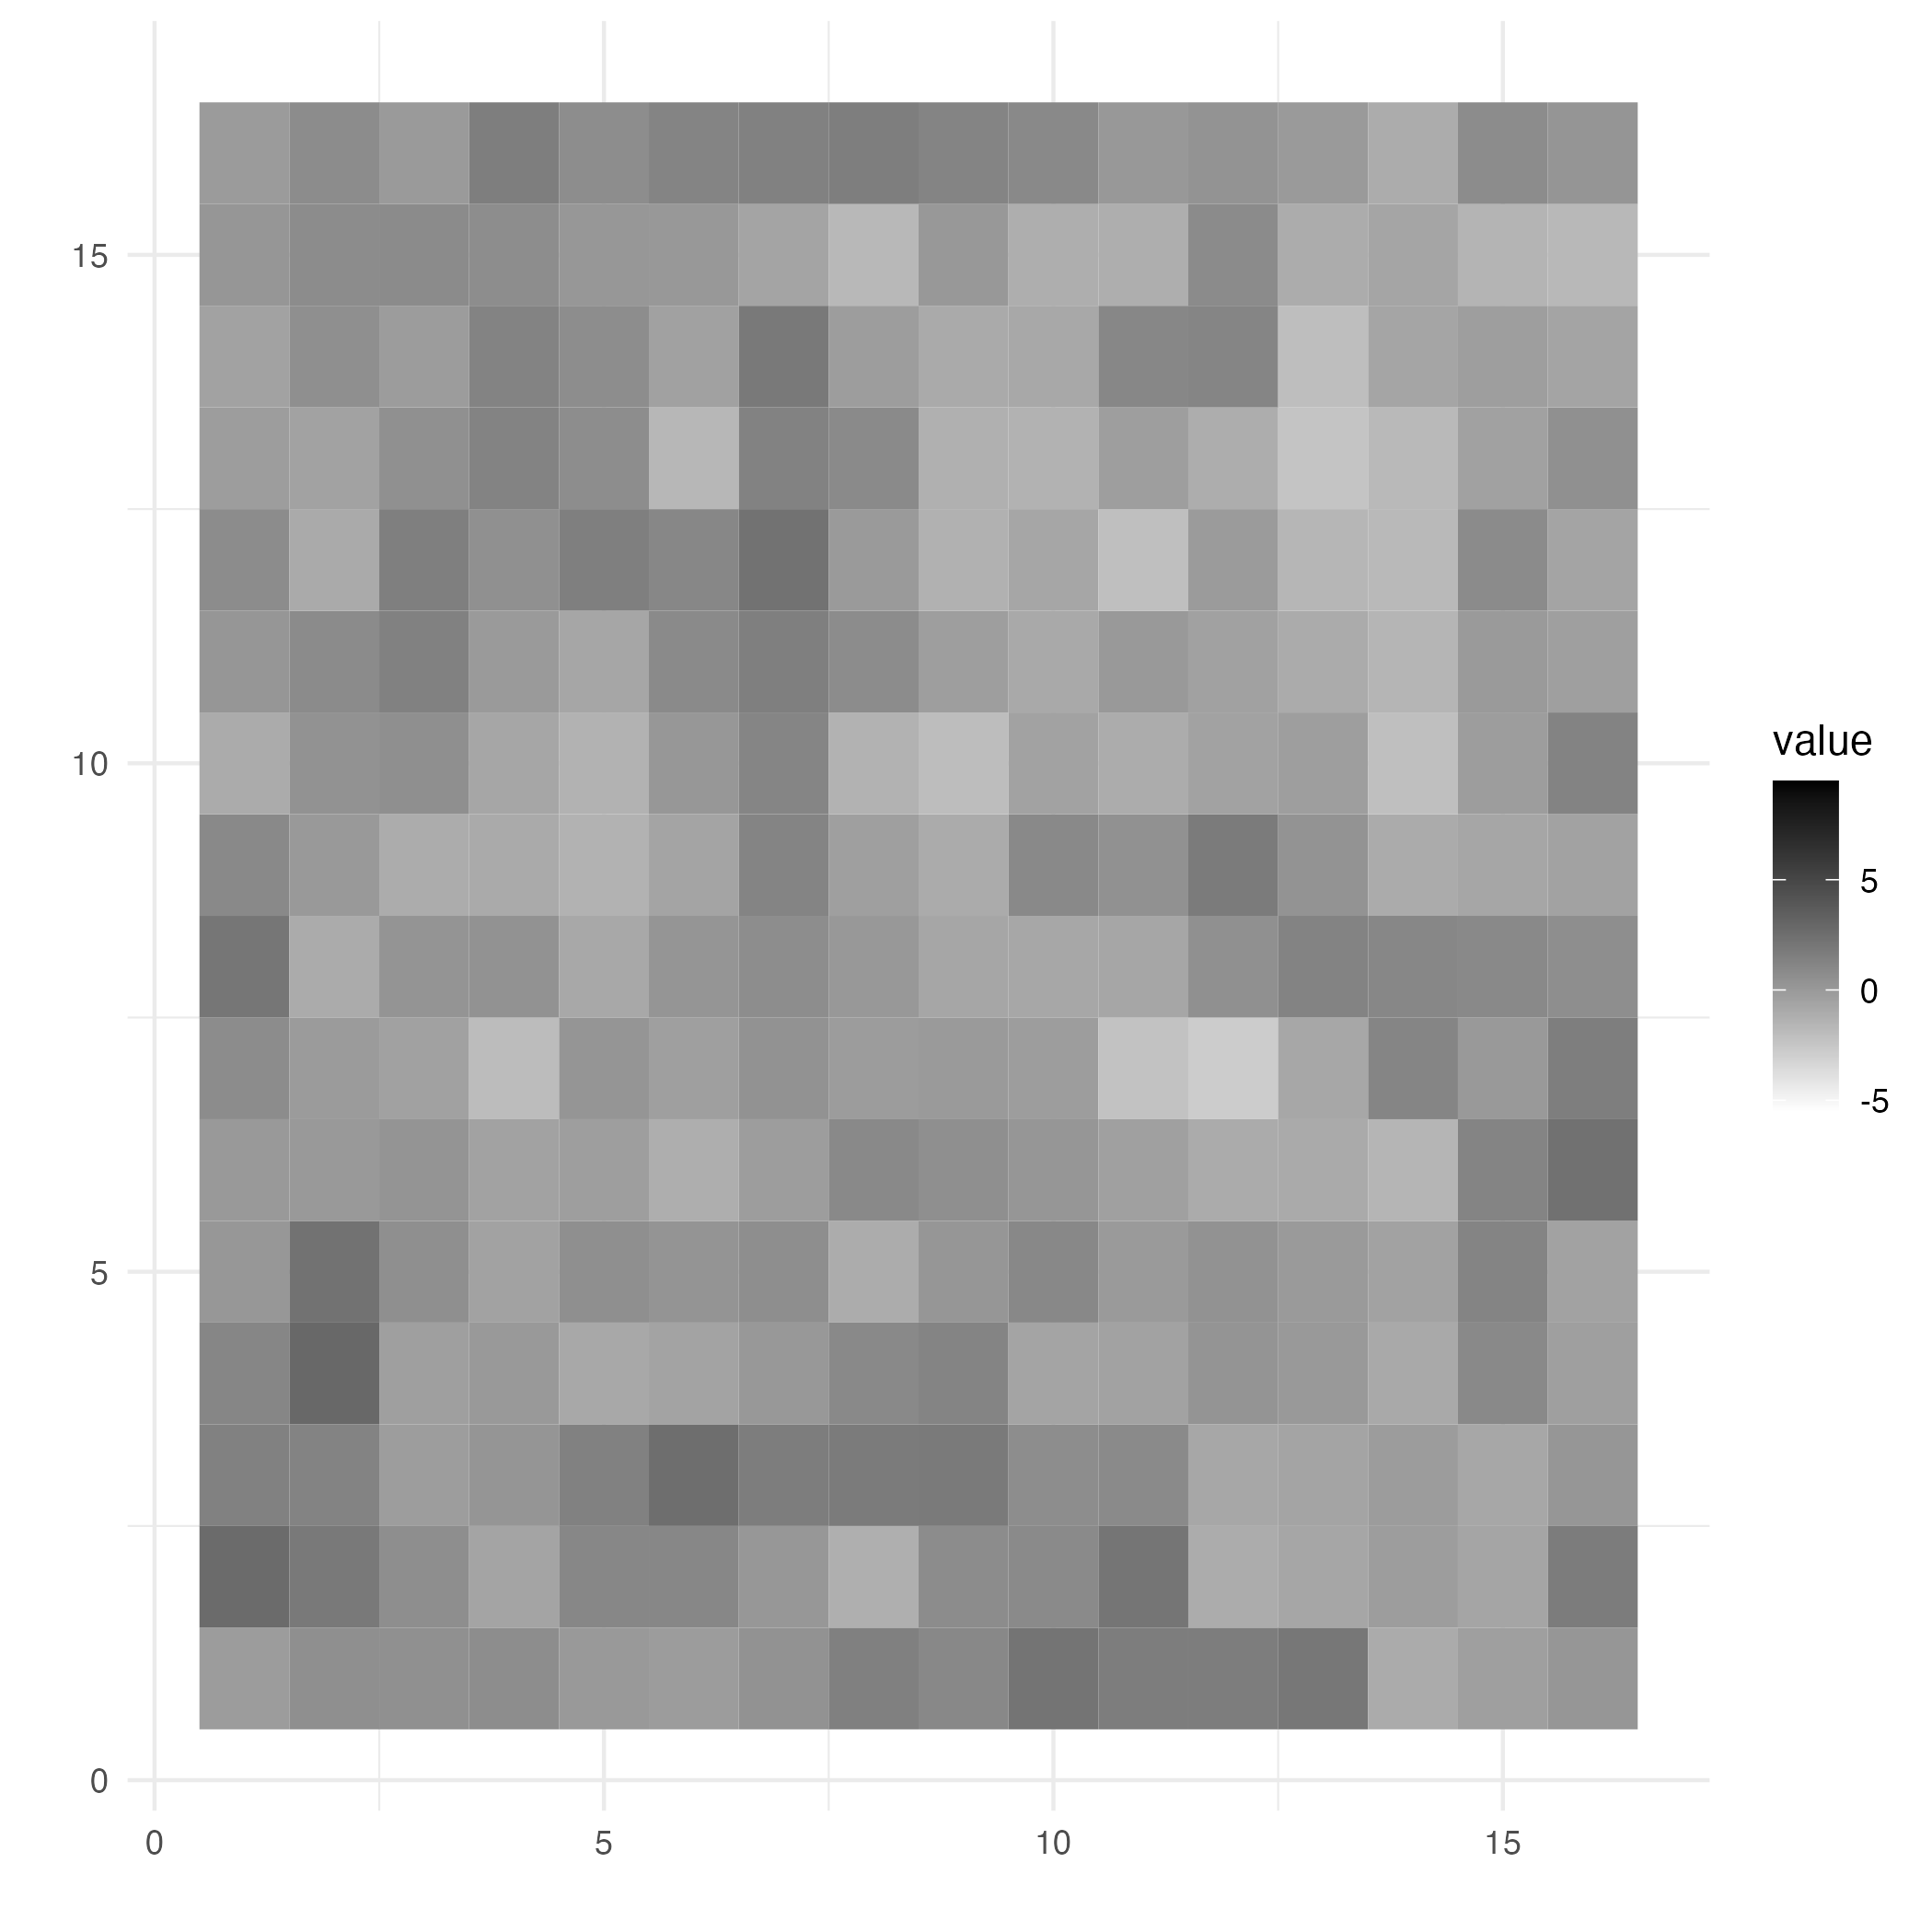
\includegraphics[width=0.9\textwidth]{../Figures/ex_image_5c.png}
    \caption{Example image without \(\beta\) effect.}
    \label{fig:image1}
  \end{minipage}\hfill
  \begin{minipage}[b]{0.45\textwidth}
    \centering
    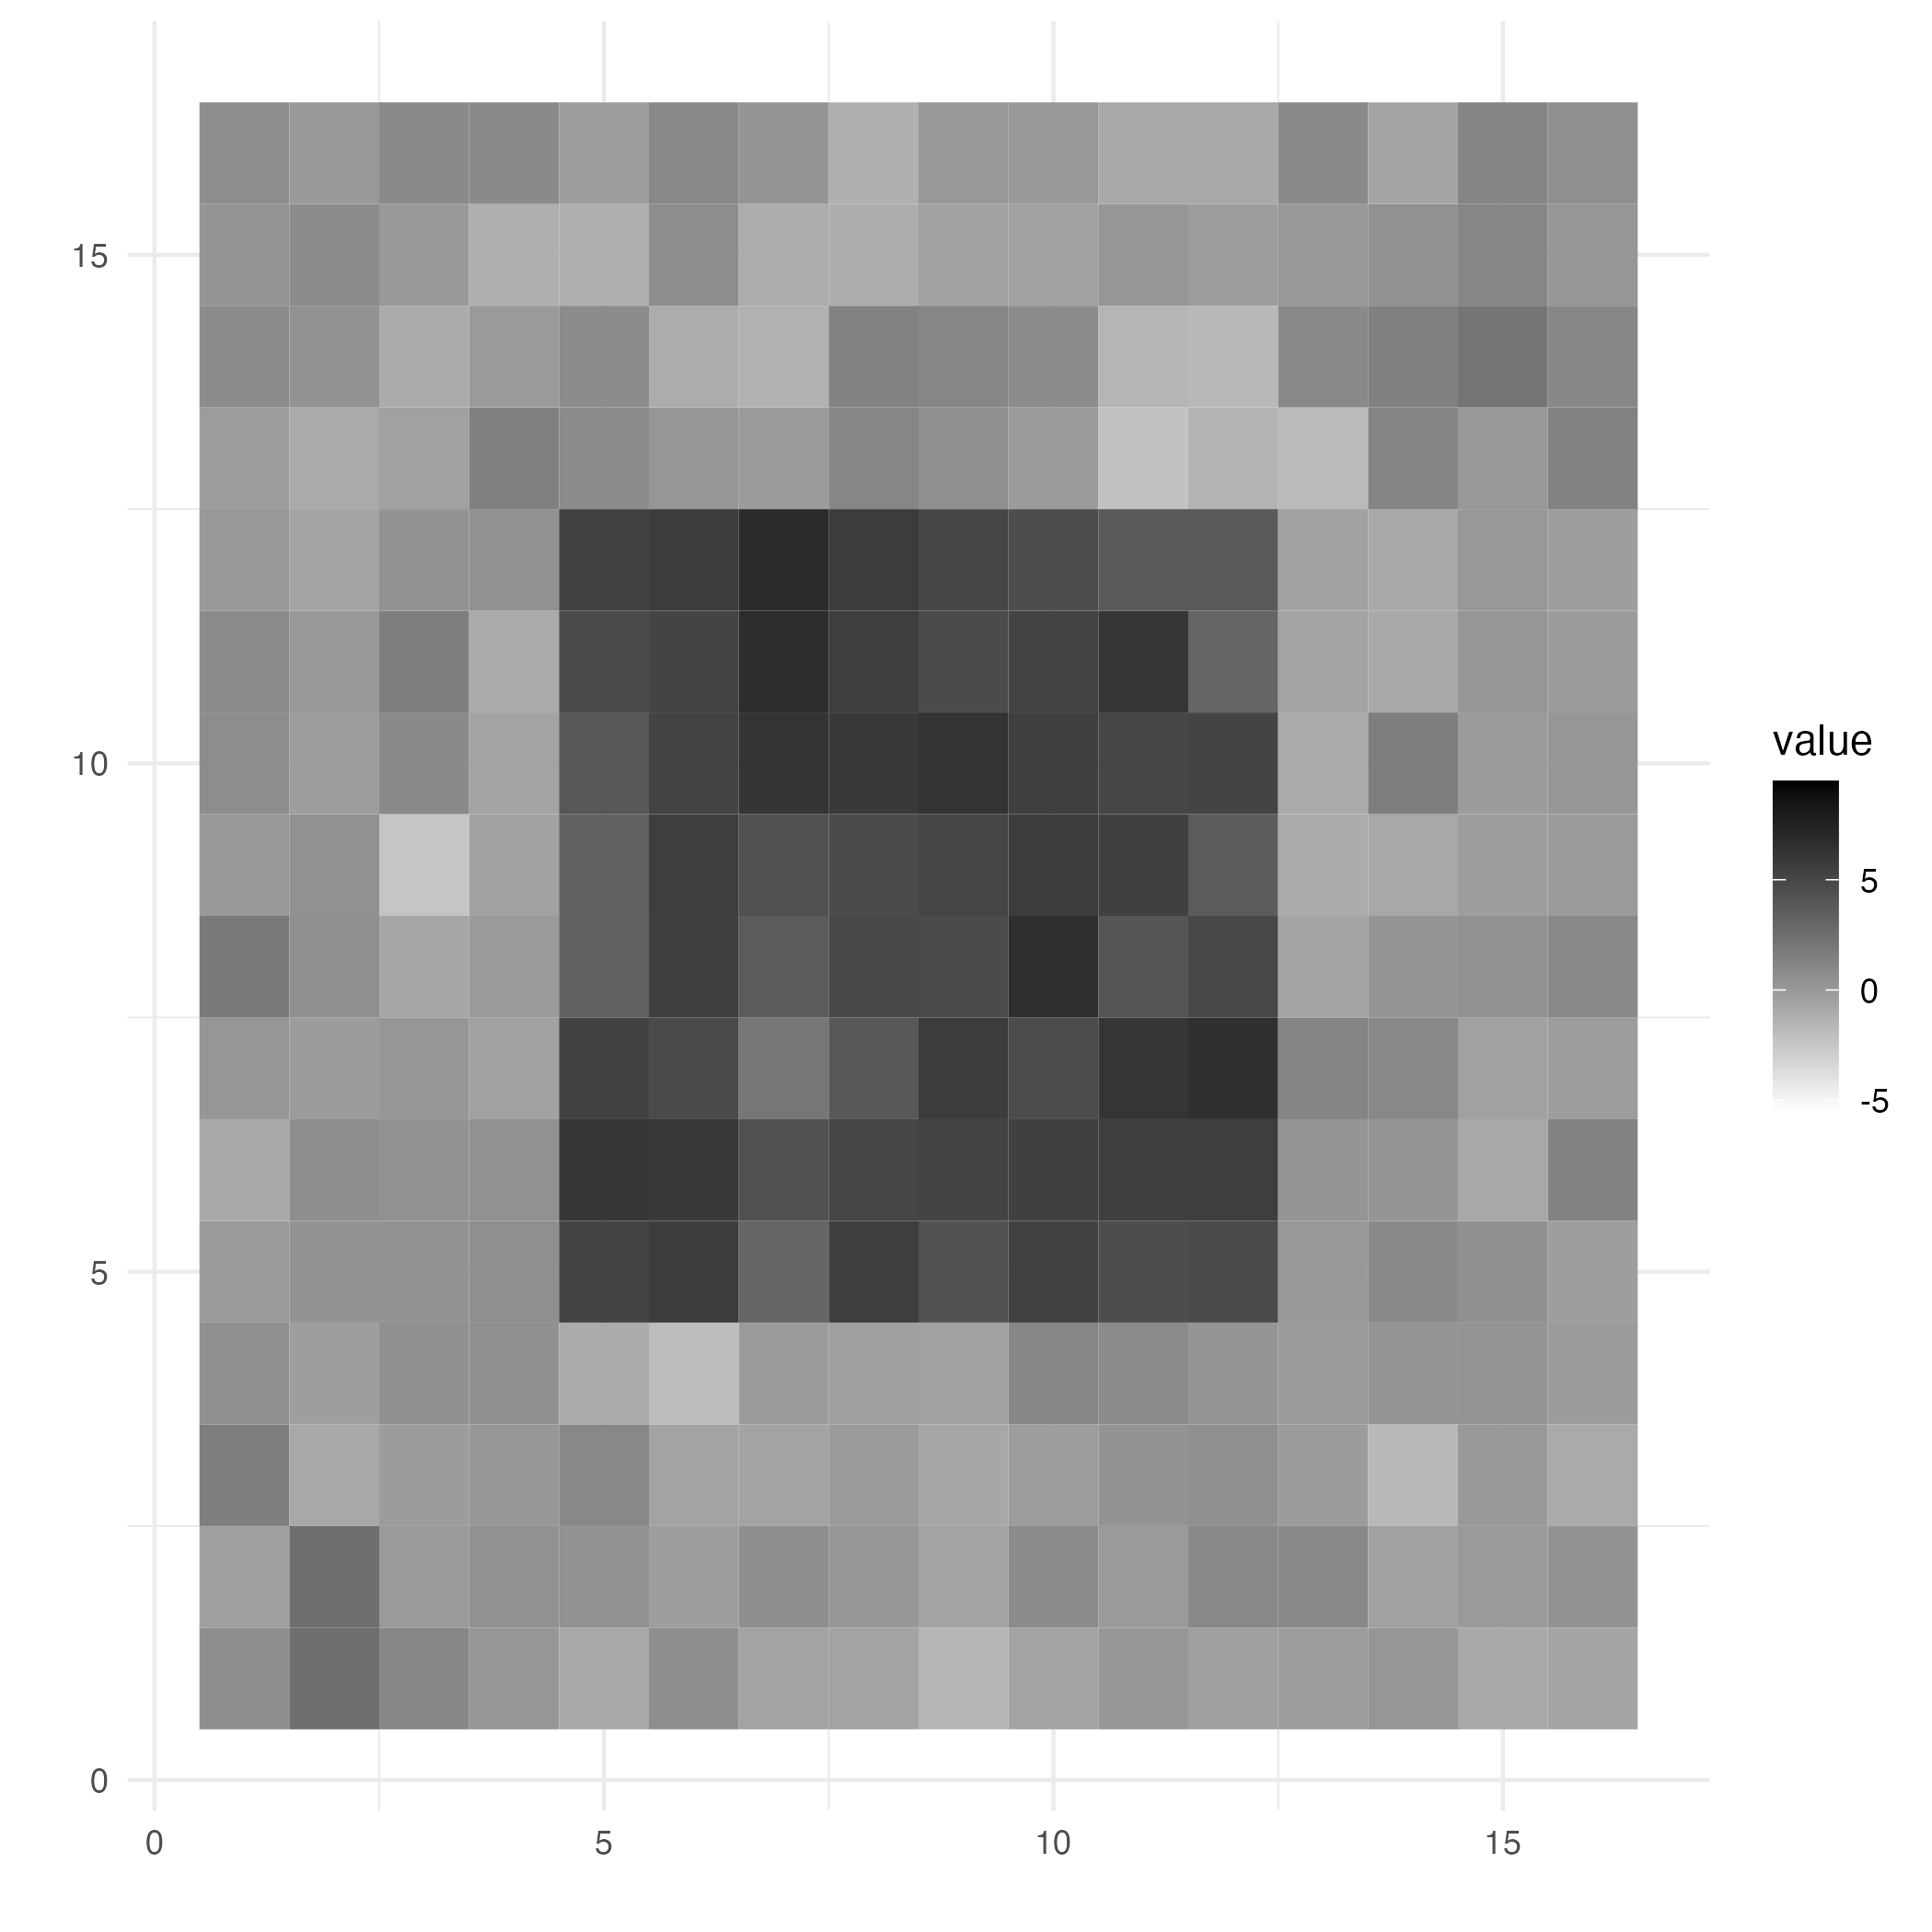
\includegraphics[width=0.9\textwidth]{../Figures/ex_image_5.png}
    \caption{Example image with \(\beta = 5\).}
    \label{fig:image2}
  \end{minipage}

  % Second Row
  \begin{minipage}[b]{0.45\textwidth}
    \centering
    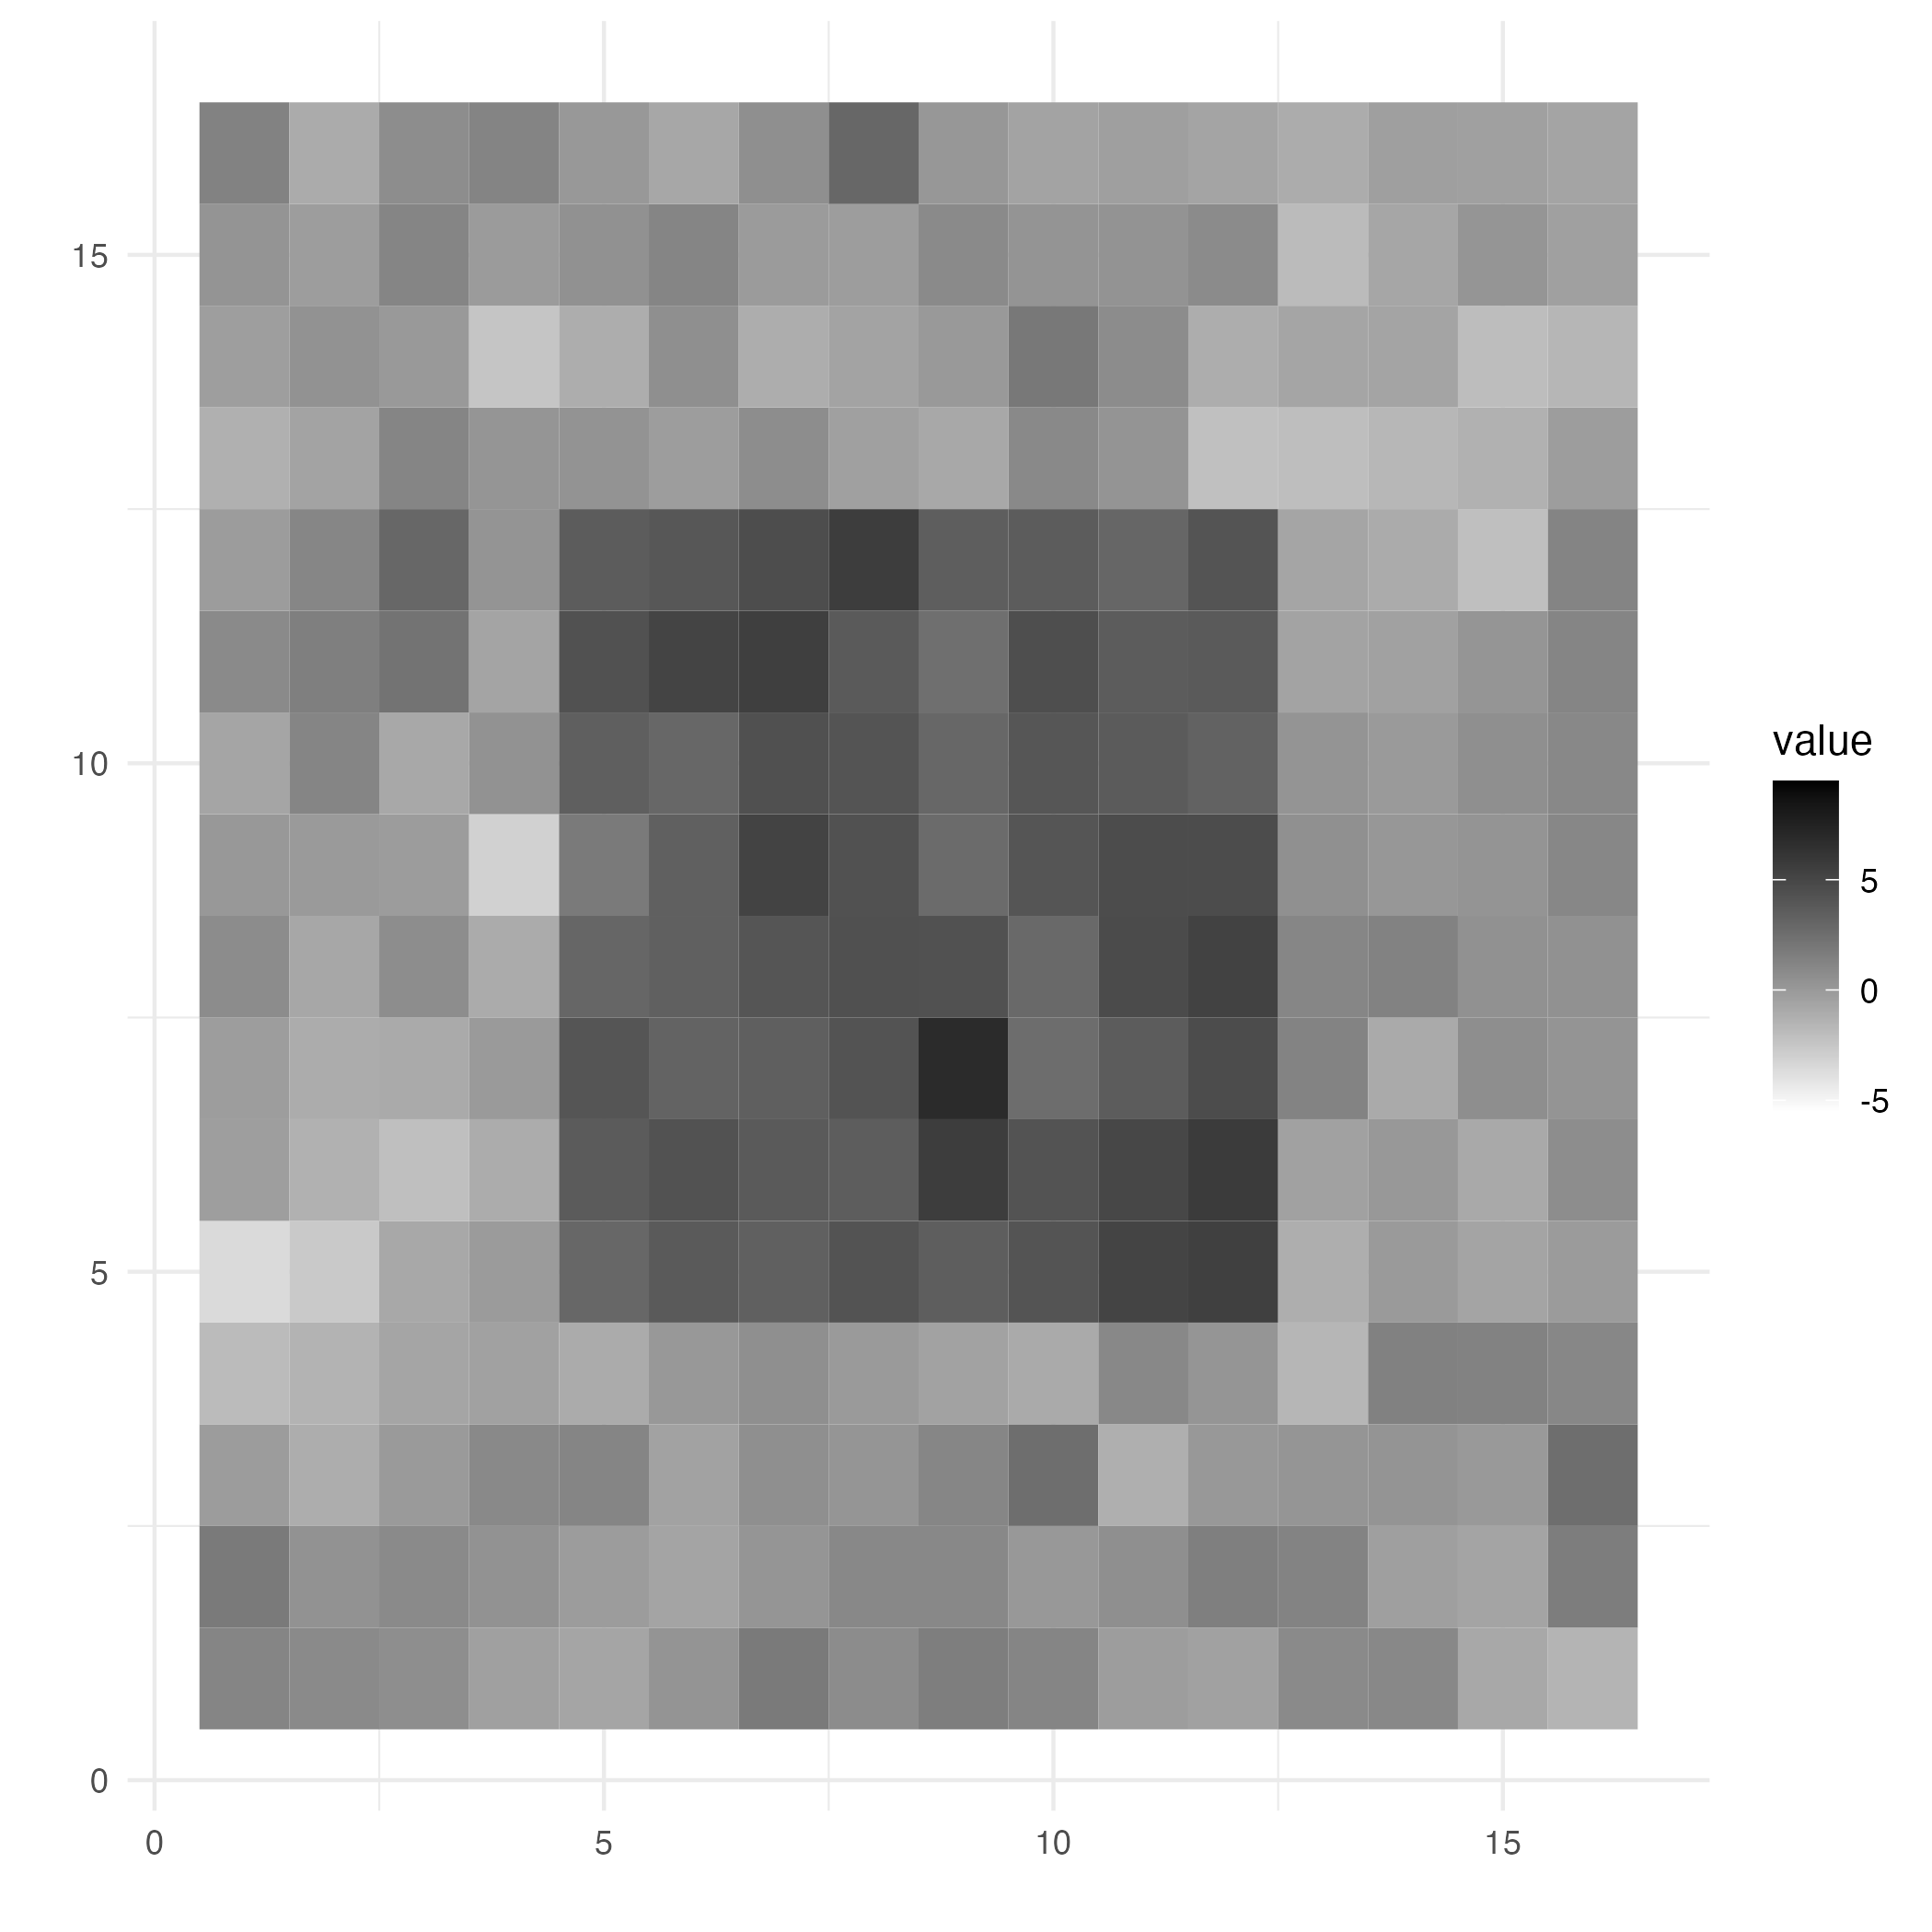
\includegraphics[width=0.9\textwidth]{../Figures/ex_image_4.png}
    \caption{Example image with \(\beta = 4\).}
    \label{fig:image3}
  \end{minipage}
\end{figure}

\section*{VBM}

In the VBM analysis, a Generalized Linear Model (GLM) was applied pixel-wise to assess group effects on pixel intensities across 1000 iterations. For each iteration, the model generated effect size estimates and p-values for each pixel. These p-values were then corrected for multiple comparisons using the Bonferroni method. Figure~\ref{fig:vbm_pvals} depicts the frequency of significant p-values in across pixels, with pixels showing significant \(\beta\) in all 100 iterations appearing in black, and those never showing significance in white.

In the VBM analysis, a Generalized Linear Model (GLM) was applied pixel-wise to assess group effects on pixel intensities across 1000 iterations. For each iteration, the model generated effect size estimates and p-values for each pixel. These p-values were then corrected for multiple comparisons using the Bonferroni method.

Figure~\ref{fig:vbm_pvals} shows the frequency of significant p-values across pixels, with pixels showing significant \( \beta \) in all 1000 iterations appearing in black, and those never showing significance in white.
Figure~\ref{fig:vbm_pvals_corr} displays the percentage of significant p-values after multiple correction.
Figure~\ref{fig:vbm_boxplots} presents a boxplot of the percentage of significant p-values in the outer (non-central) areas, with the left boxplot showing values before adjustment and the right boxplot showing values after adjustment.

\begin{figure}[h]
  \centering
  % First figure
  \begin{minipage}[b]{0.45\textwidth}
    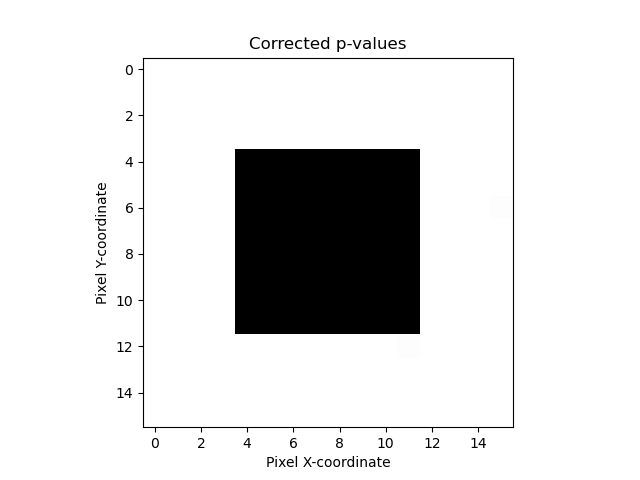
\includegraphics[width=\textwidth]{/Users/siyangren/Documents/ra-cida/ESFGSP_Paper/Figures/vbm_pvals.png}
    \caption{Percentage of significant p-values across pixels in VBM analysis.}
    \label{fig:vbm_pvals}
  \end{minipage}
  \hfill % This command adds a space between the two figures
  % Second figure
  \begin{minipage}[b]{0.45\textwidth}
    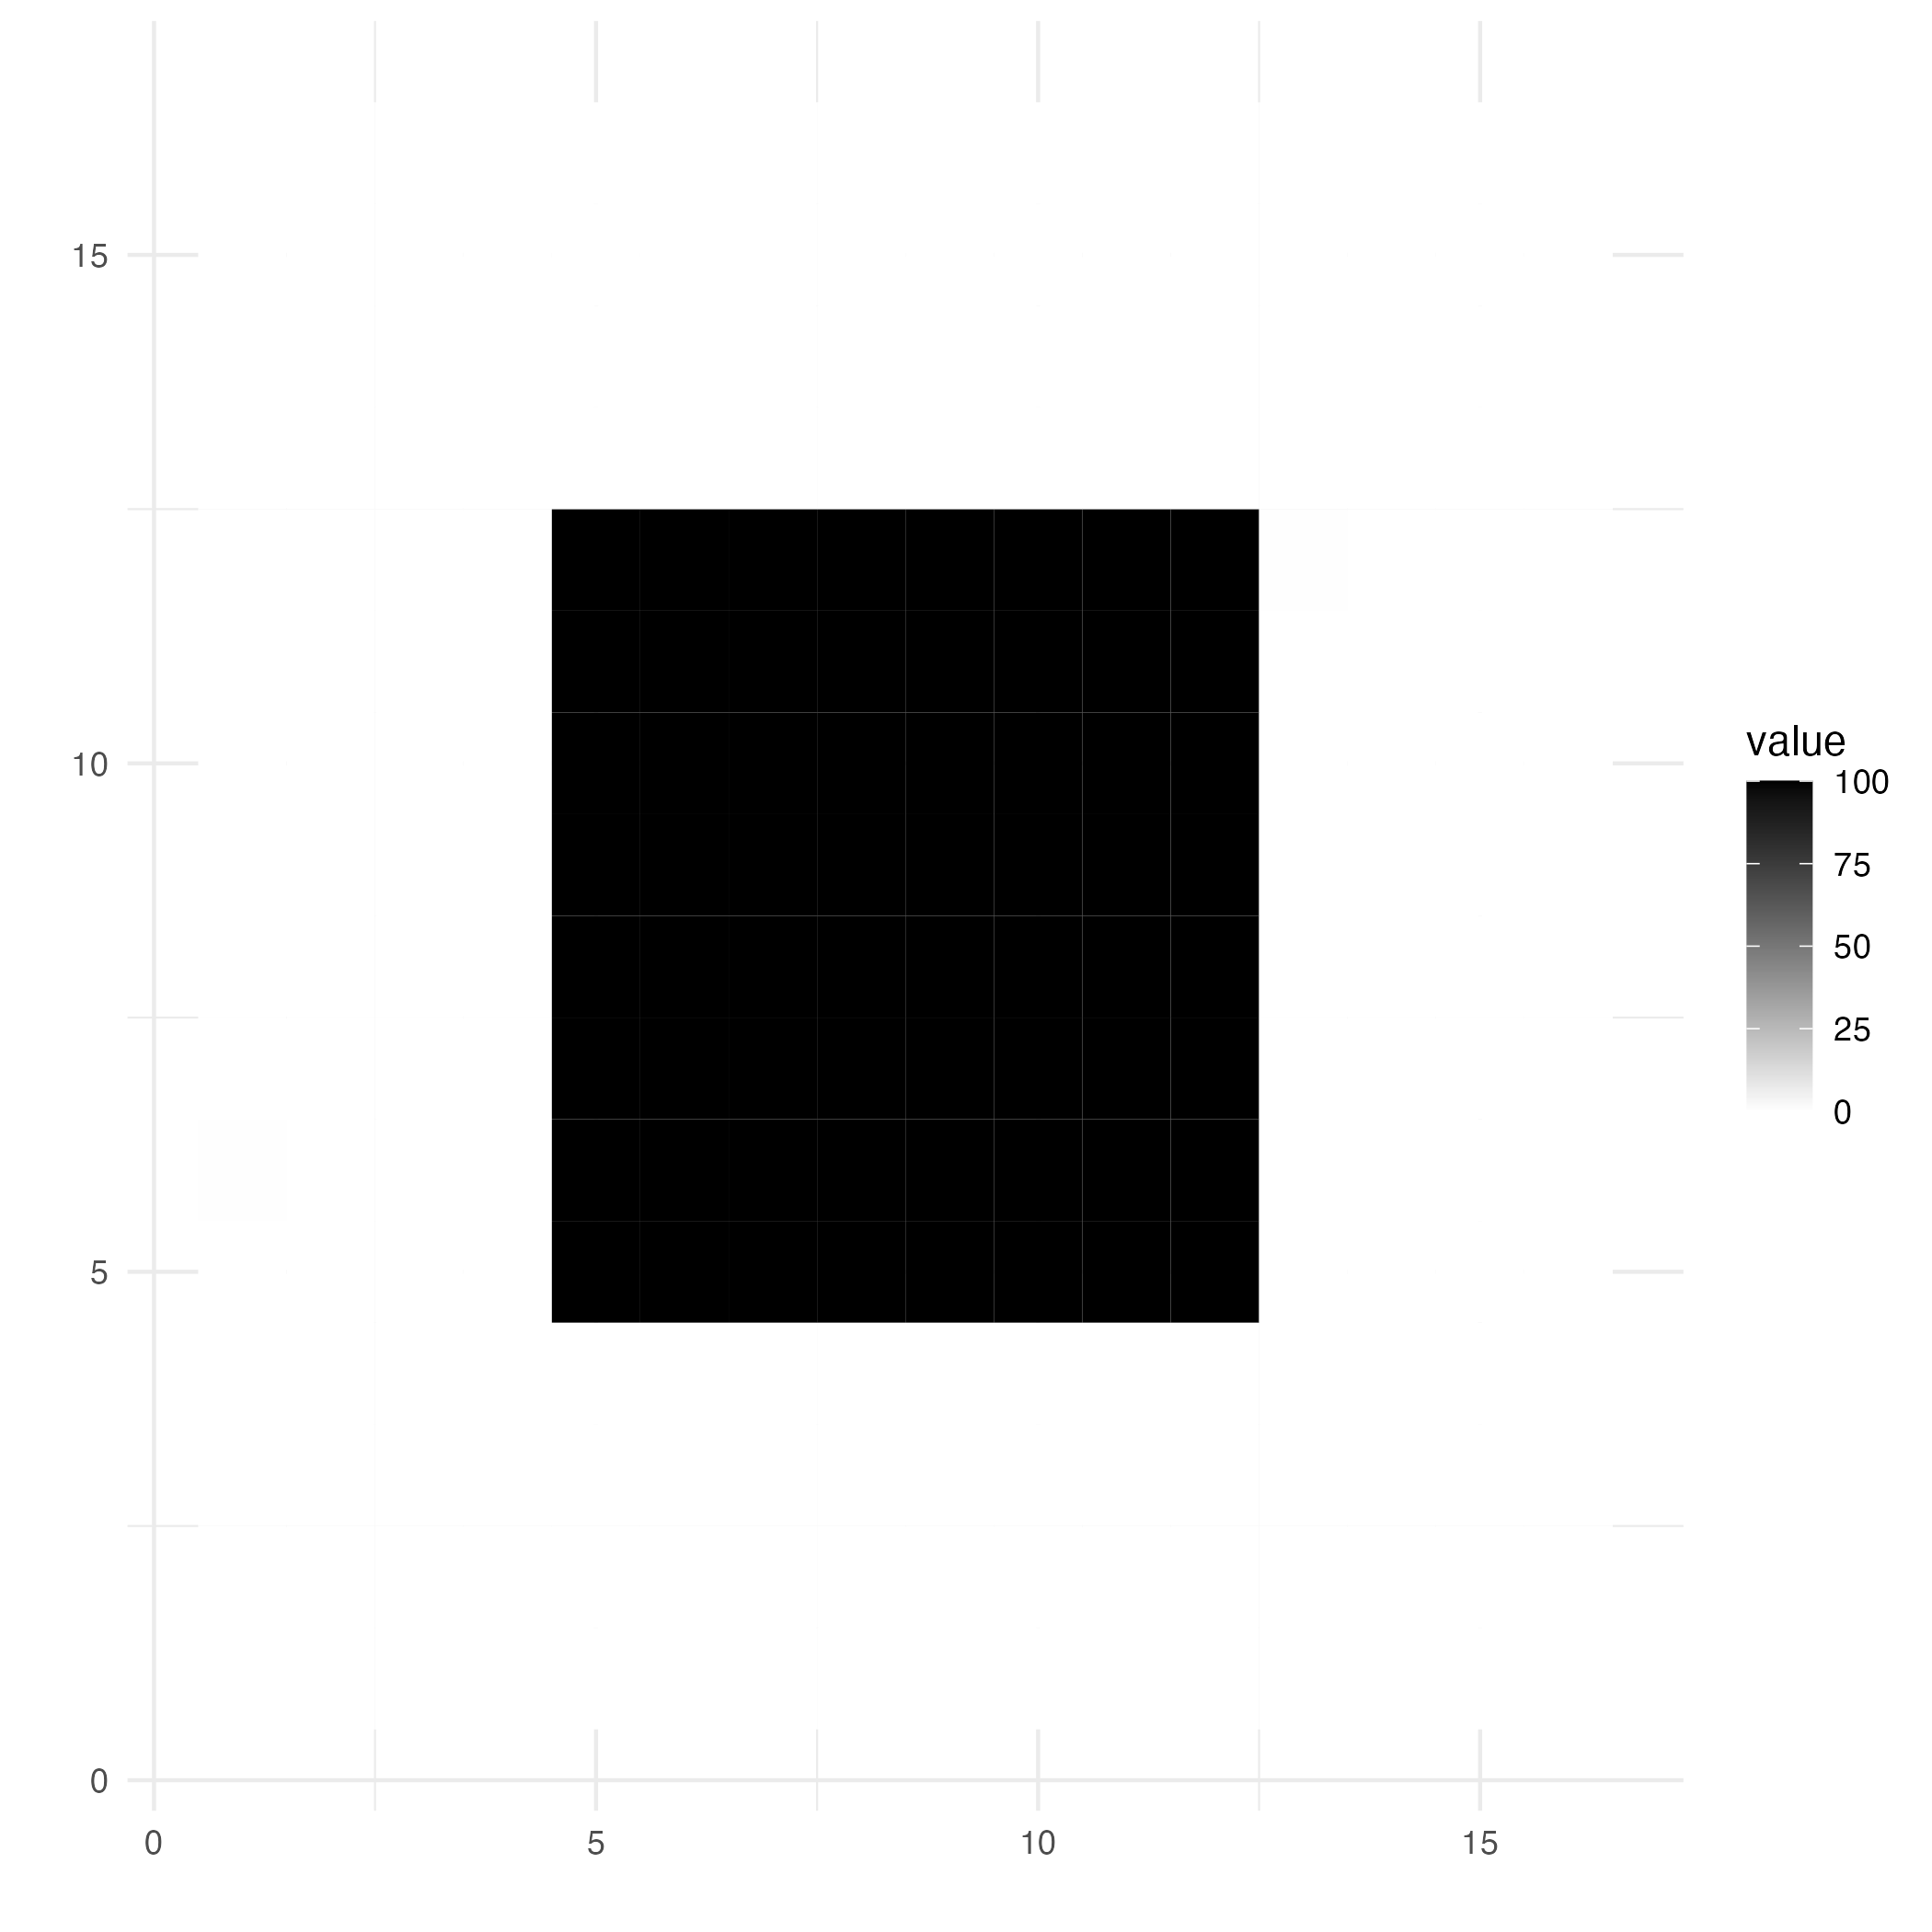
\includegraphics[width=\textwidth]{/Users/siyangren/Documents/ra-cida/ESFGSP_Paper/Figures/vbm_pvals_corr.png}
    \caption{Percentage of significant p-values after correction across pixels in VBM analysis.}
    \label{fig:vbm_pvals_corr}
  \end{minipage}
\end{figure}

\begin{figure}[h]
  \centering
  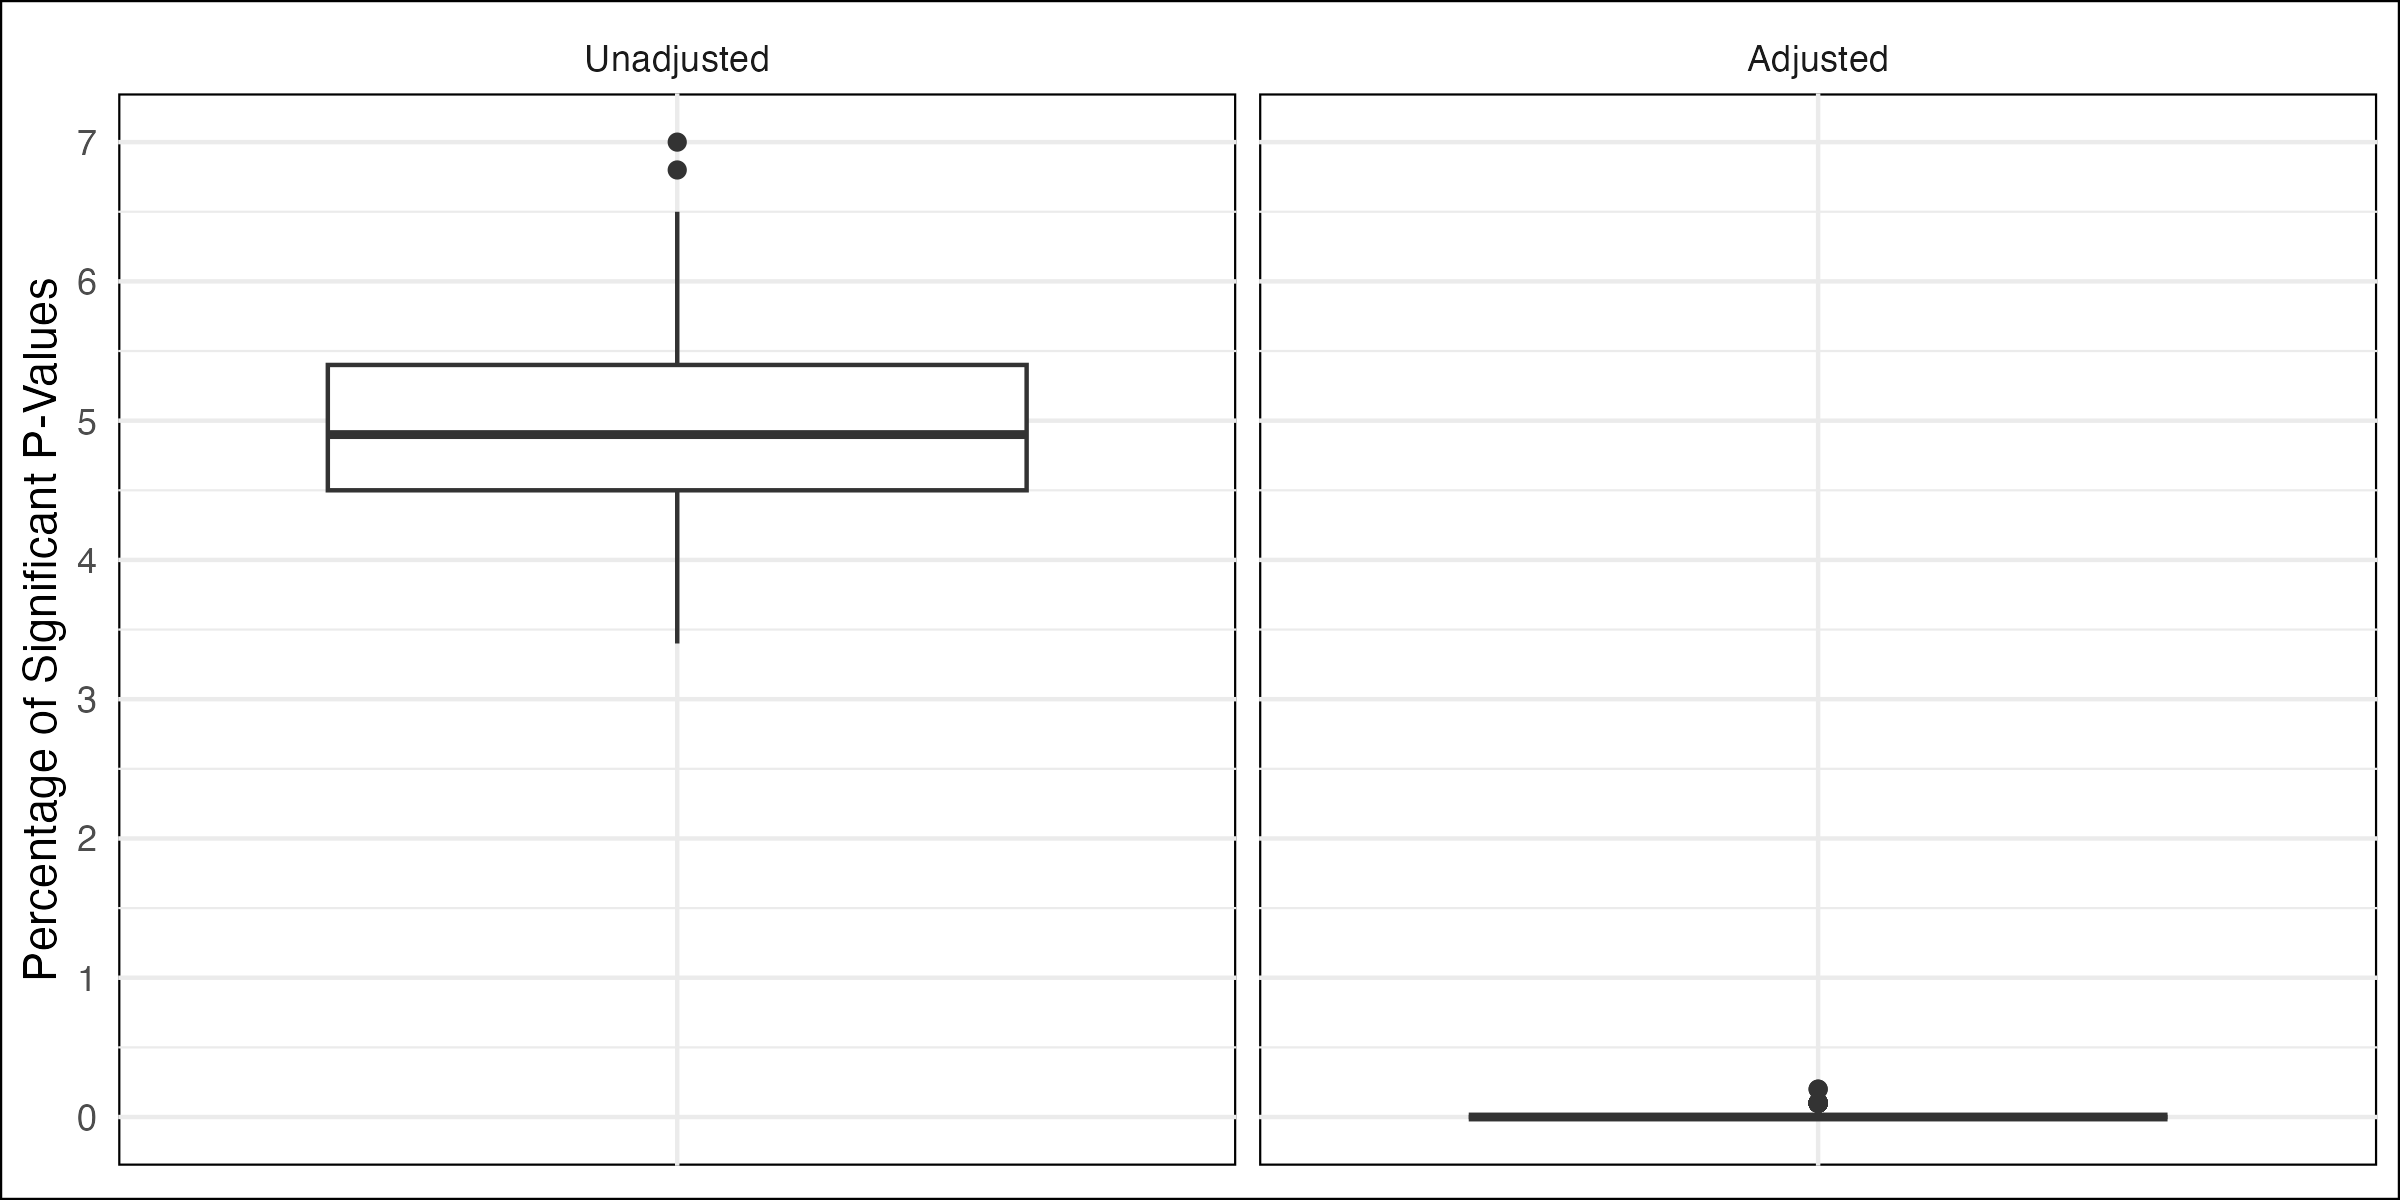
\includegraphics[width=0.7\textwidth]{../Figures/vbm_boxplots.png}
  \caption{Percentage of significant p-values in outer area before (left) and after (right) adjustment from the VBM analysis.}
  \label{fig:vbm_boxplots}
\end{figure}


% \section*{spVBM}

% The spVBM model is:
% \[
%     \begin{aligned}
%          & y_s^i=\sum_{k=1}^K x_{s, k}^i \beta_{s, k}^{S V C}+\mathbf{Z}^{\mathbf{i}} \mathbf{b}^{\mathbf{i}}+\varepsilon_s^i                                                                                                                      \\
%          & \beta_{s, k}^{S V C}=\beta_k+[\mathbf{E} \Gamma]_{s, k}                                                                                                                                                                                 \\
%          & \mathbf{b}^{\mathbf{i}} \sim \mathcal{N}(\mathbf{0}, G), \quad \varepsilon_i \sim \mathcal{N}\left(0, \sigma^2\right), \quad \Gamma_{, k} \sim \mathcal{N}\left(\mathbf{0}, \sigma_k^2 \boldsymbol{\Lambda}\left(\alpha_k\right)\right)
%     \end{aligned}
% \]
% \(y_s^i\) denote the spatial outcome for subject \(i\) voxel \(s\). \(\mathbf{Z}\) denote non-spatial subject-level covariates for non-spatial random effects.

% In our simulated data, this could be simplified to \(y_s^i = x_s^i \beta_s^{SVC} + (?) \). My question is, which term captures the exponential correlation structure in the model? \(G\) or \(\Gamma\)?

% \begin{figure}[H]
%     \centering
%     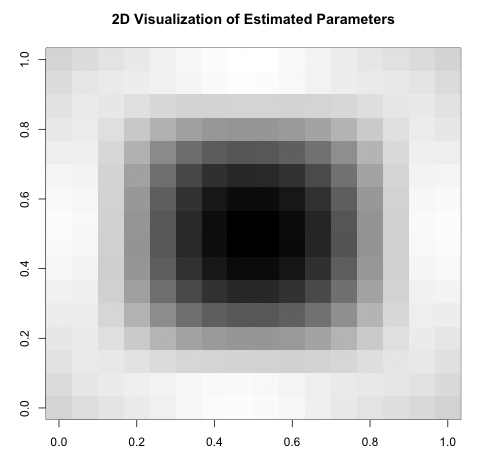
\includegraphics[width=0.5\textwidth]{/Users/siyangren/Documents/ra-cida/ESFGSP_Paper/Figures/spvbm_coefs_april_3.png}
%     \caption{Estimated coefficients}
%     \label{fig:my_label}
% \end{figure}

\section*{LASSO}

A LASSO model was employed to predict group assignments using pixel values from images. In each iteration, 80\% of the data was used for training and the remaining 20\% for testing. The optimal \(\lambda\) parameters, \texttt{lambda\_min} and \texttt{lambda\_1se}, were determined via cross-validation within the training group. The model's performance was assessed on the test group using accuracy and AUC metrics.

Initially, including all pixel values in the model led to perfect separation, indicating potential overfitting. To address this, the model construction began by incrementally adding one pixel from the image's edge and one from the center, evaluating if these additions achieved perfect accuracy. After integrating two pixels from each area, totaling four pixels, the model achieved perfect separation.

Additionally, a permutation test was conducted to estimate p-values. Using all the pixels, 500 iterations were performed. Within each iteration, the outcome was permuted 100 times. The original coefficients were compared with the permuted coefficient estimates to simulate the p-values of each covariate/pixel.

Figures~\ref{fig:lasso_pvals}, \ref{fig:lasso_pvals_corr}, and \ref{fig:lasso_boxplot} illustrate the results of the analysis:
\begin{itemize}
  \item Figure~\ref{fig:lasso_pvals} shows the p-values before multiple adjustment.
  \item Figure~\ref{fig:lasso_pvals_corr} displays the p-values after multiple adjustment.
  \item Figure~\ref{fig:lasso_boxplot} presents a boxplot of the percentage of significant p-values for the outer area before and after adjustment.
\end{itemize}


\begin{figure}[h]
  \centering
  % First figure
  \begin{minipage}[b]{0.45\textwidth}
    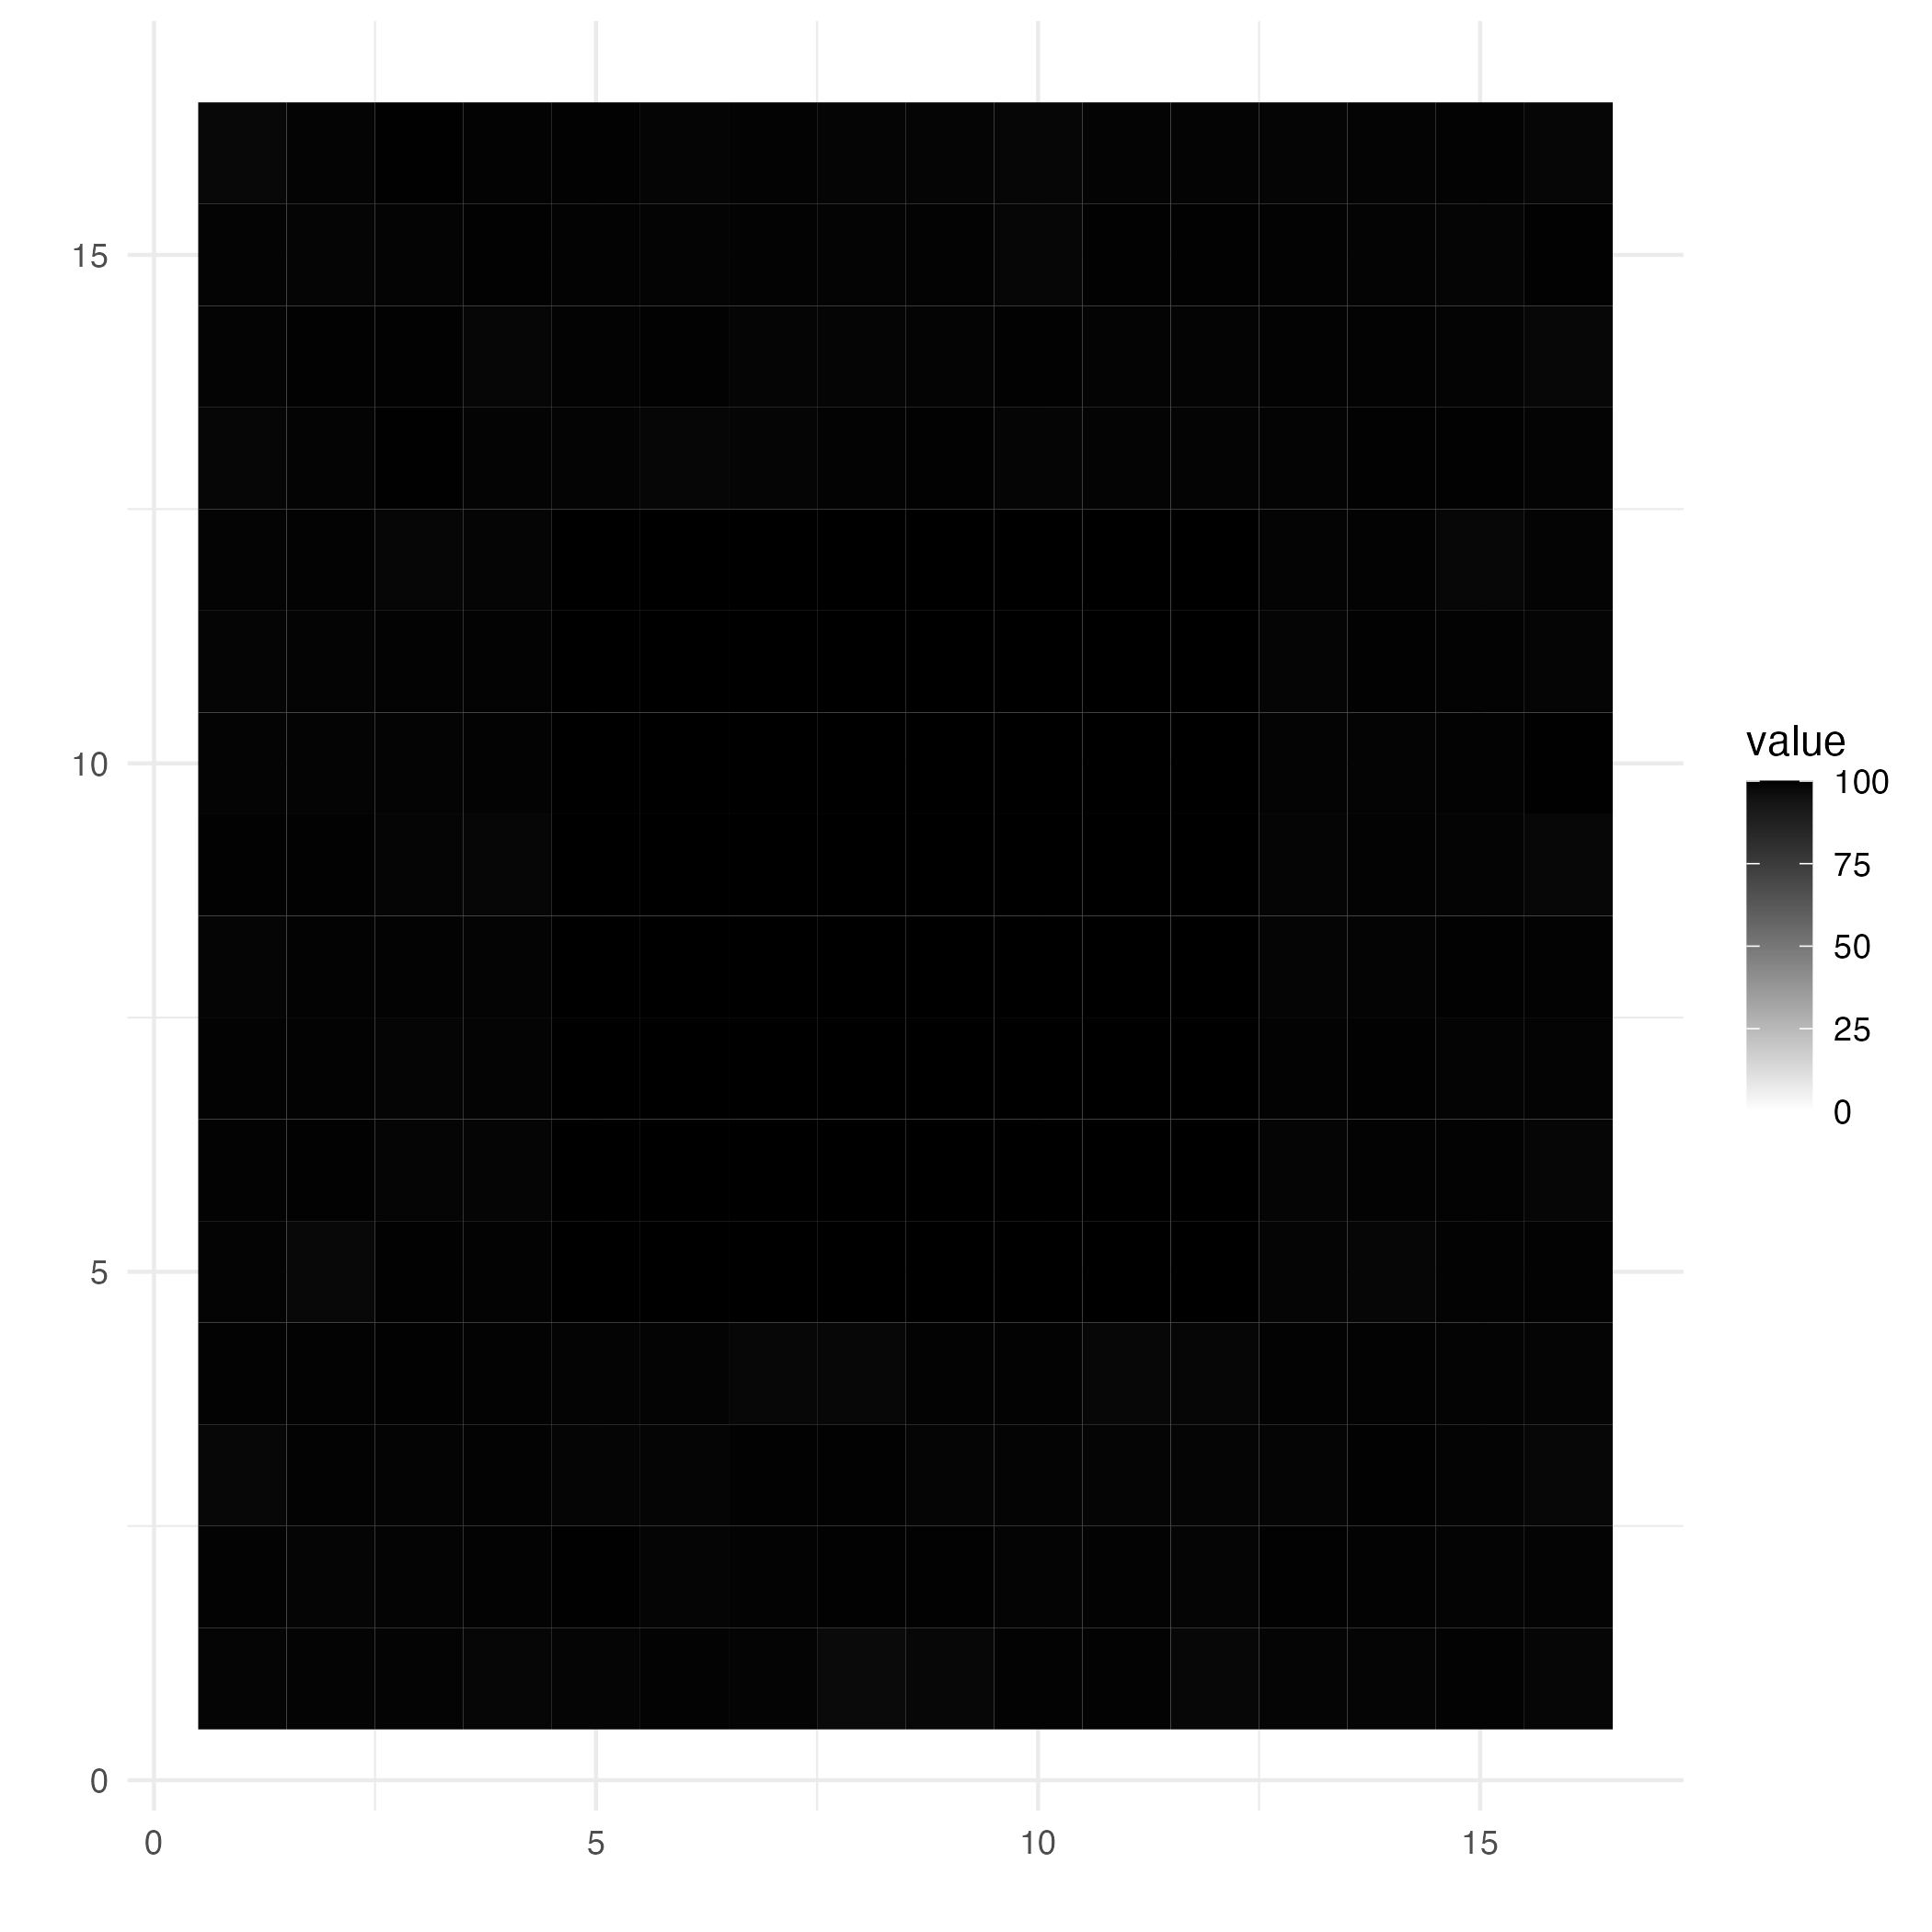
\includegraphics[width=\textwidth]{/Users/siyangren/Documents/ra-cida/ESFGSP_Paper/Figures/lasso_pvals.png}
    \caption{Percentage of significant p-values across pixels in LASSO.}
    \label{fig:lasso_pvals}
  \end{minipage}
  \hfill % This command adds a space between the two figures
  % Second figure
  \begin{minipage}[b]{0.45\textwidth}
    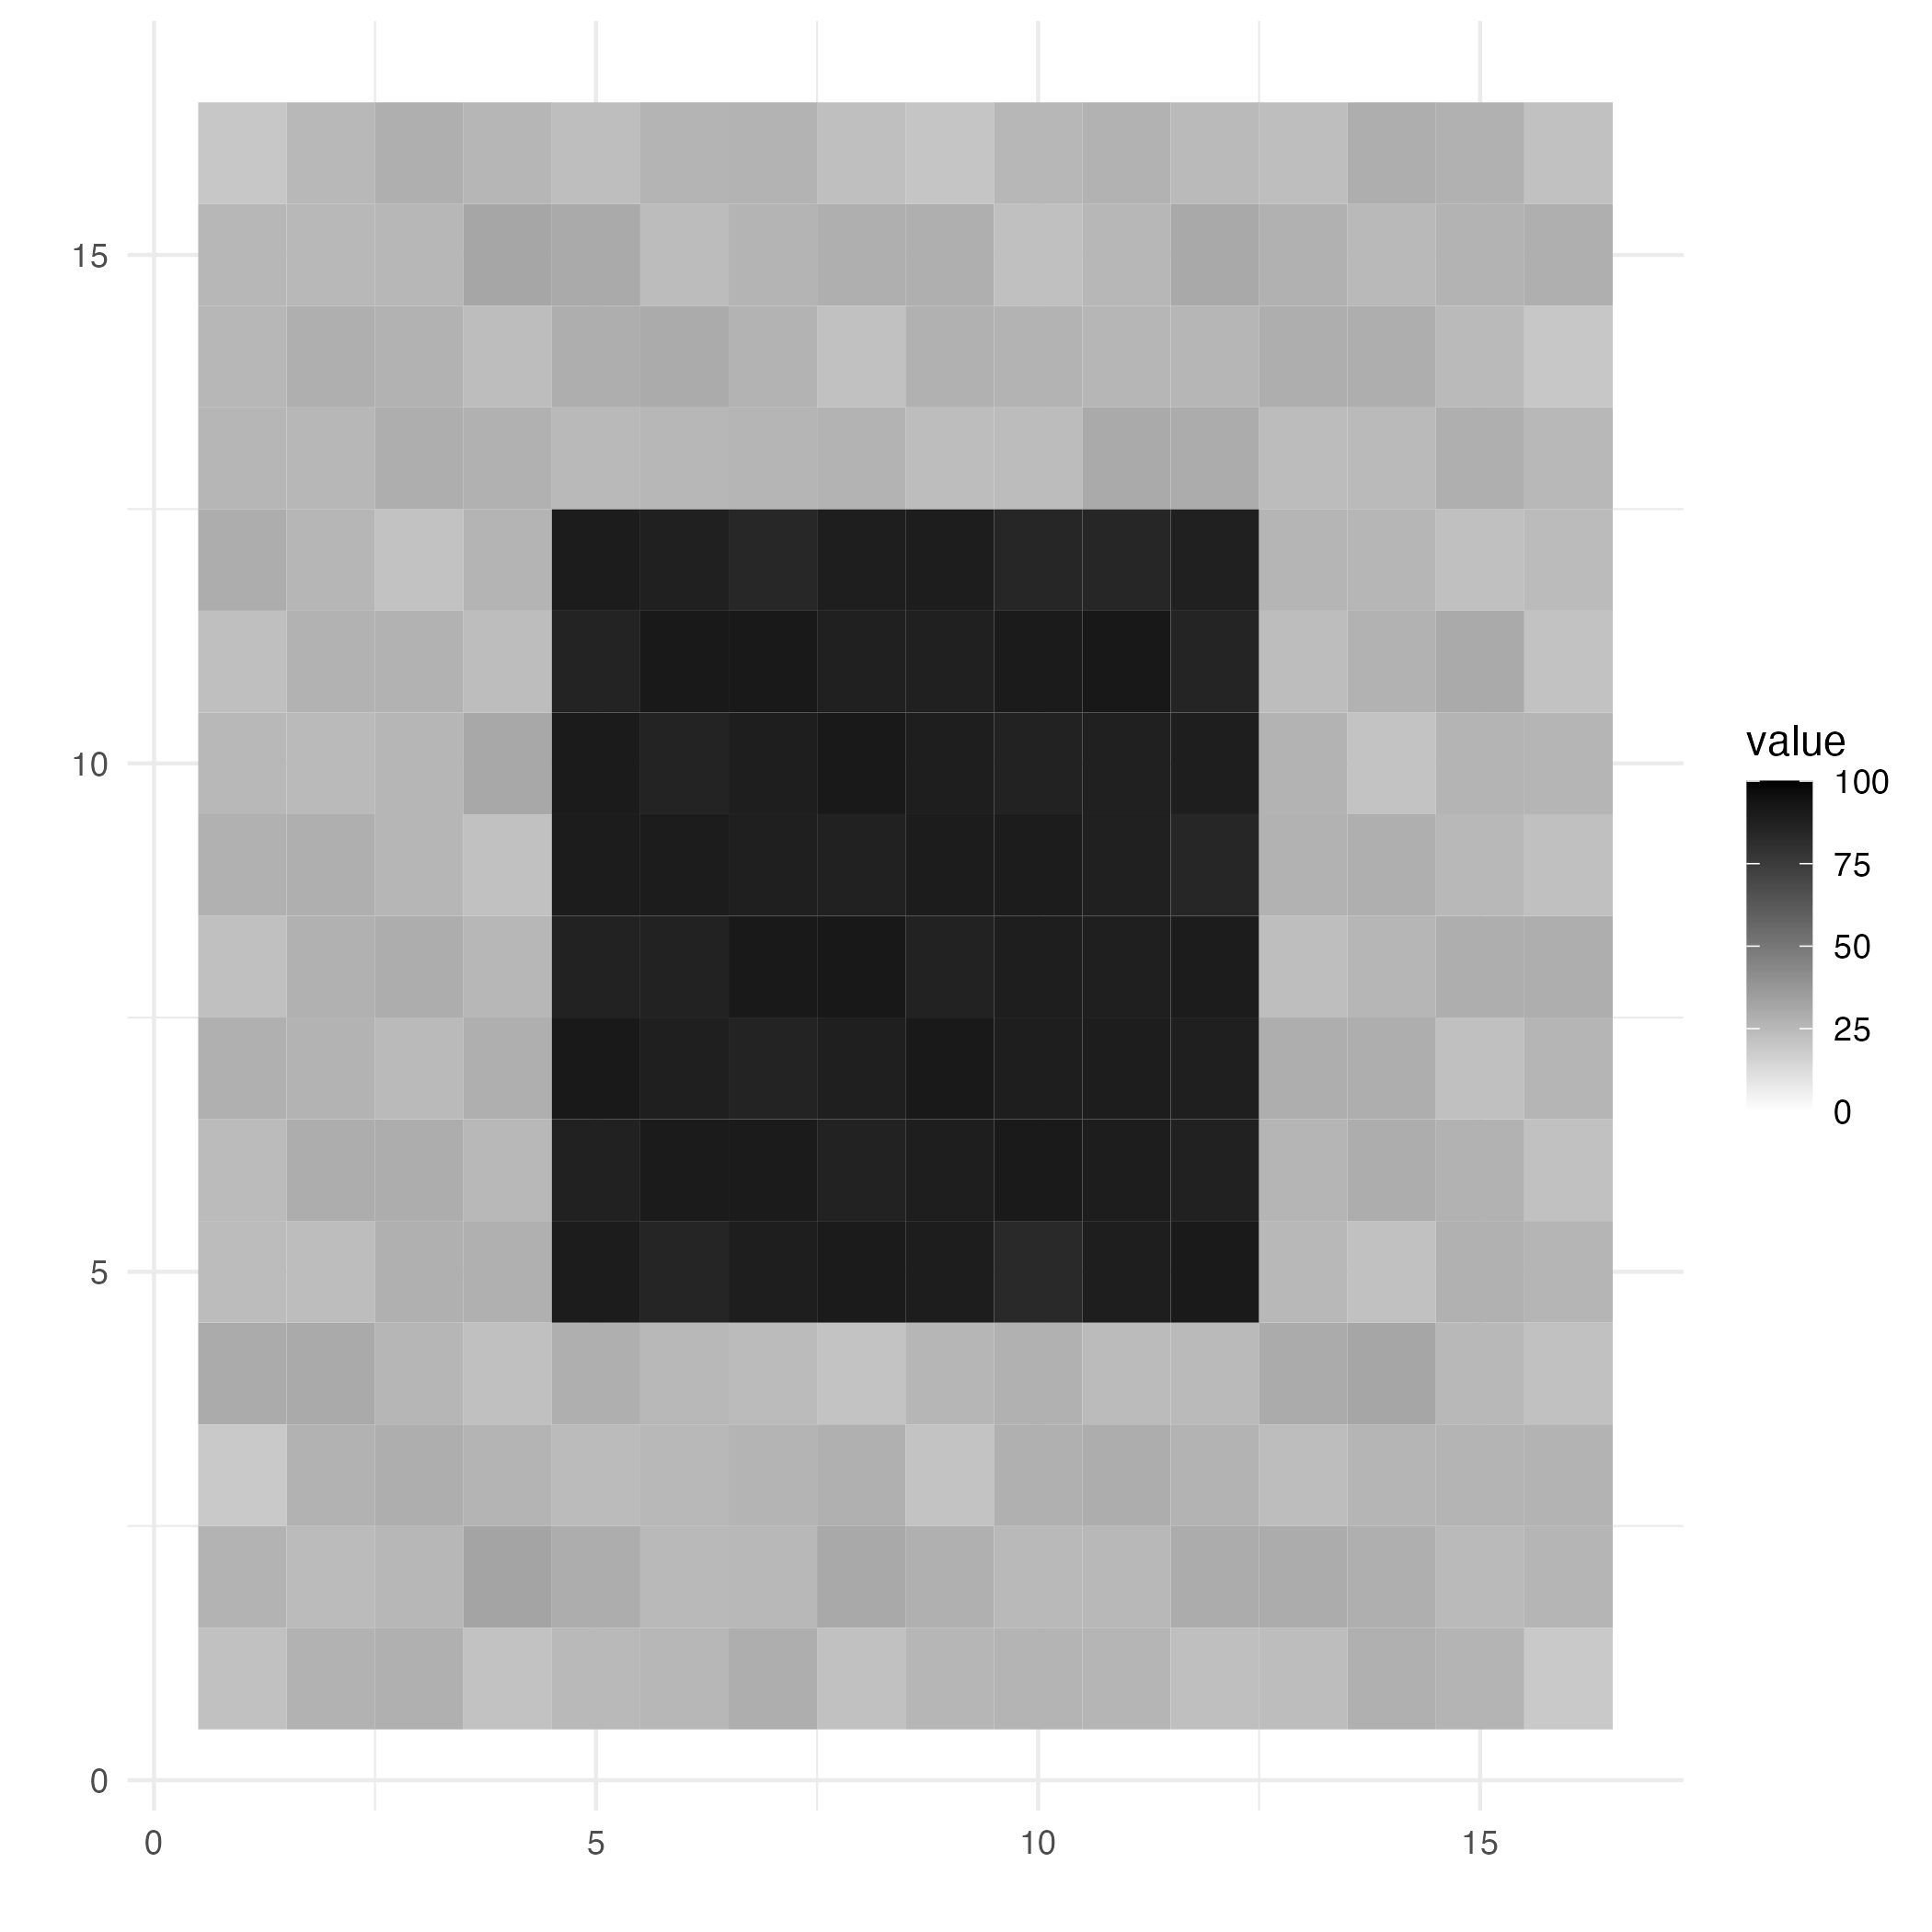
\includegraphics[width=\textwidth]{/Users/siyangren/Documents/ra-cida/ESFGSP_Paper/Figures/lasso_pvals_corr.png}
    \caption{Percentage of significant p-values after correction across pixels in LASSO.}
    \label{fig:lasso_pvals_corr}
  \end{minipage}
\end{figure}

\begin{figure}[h]
  \centering
  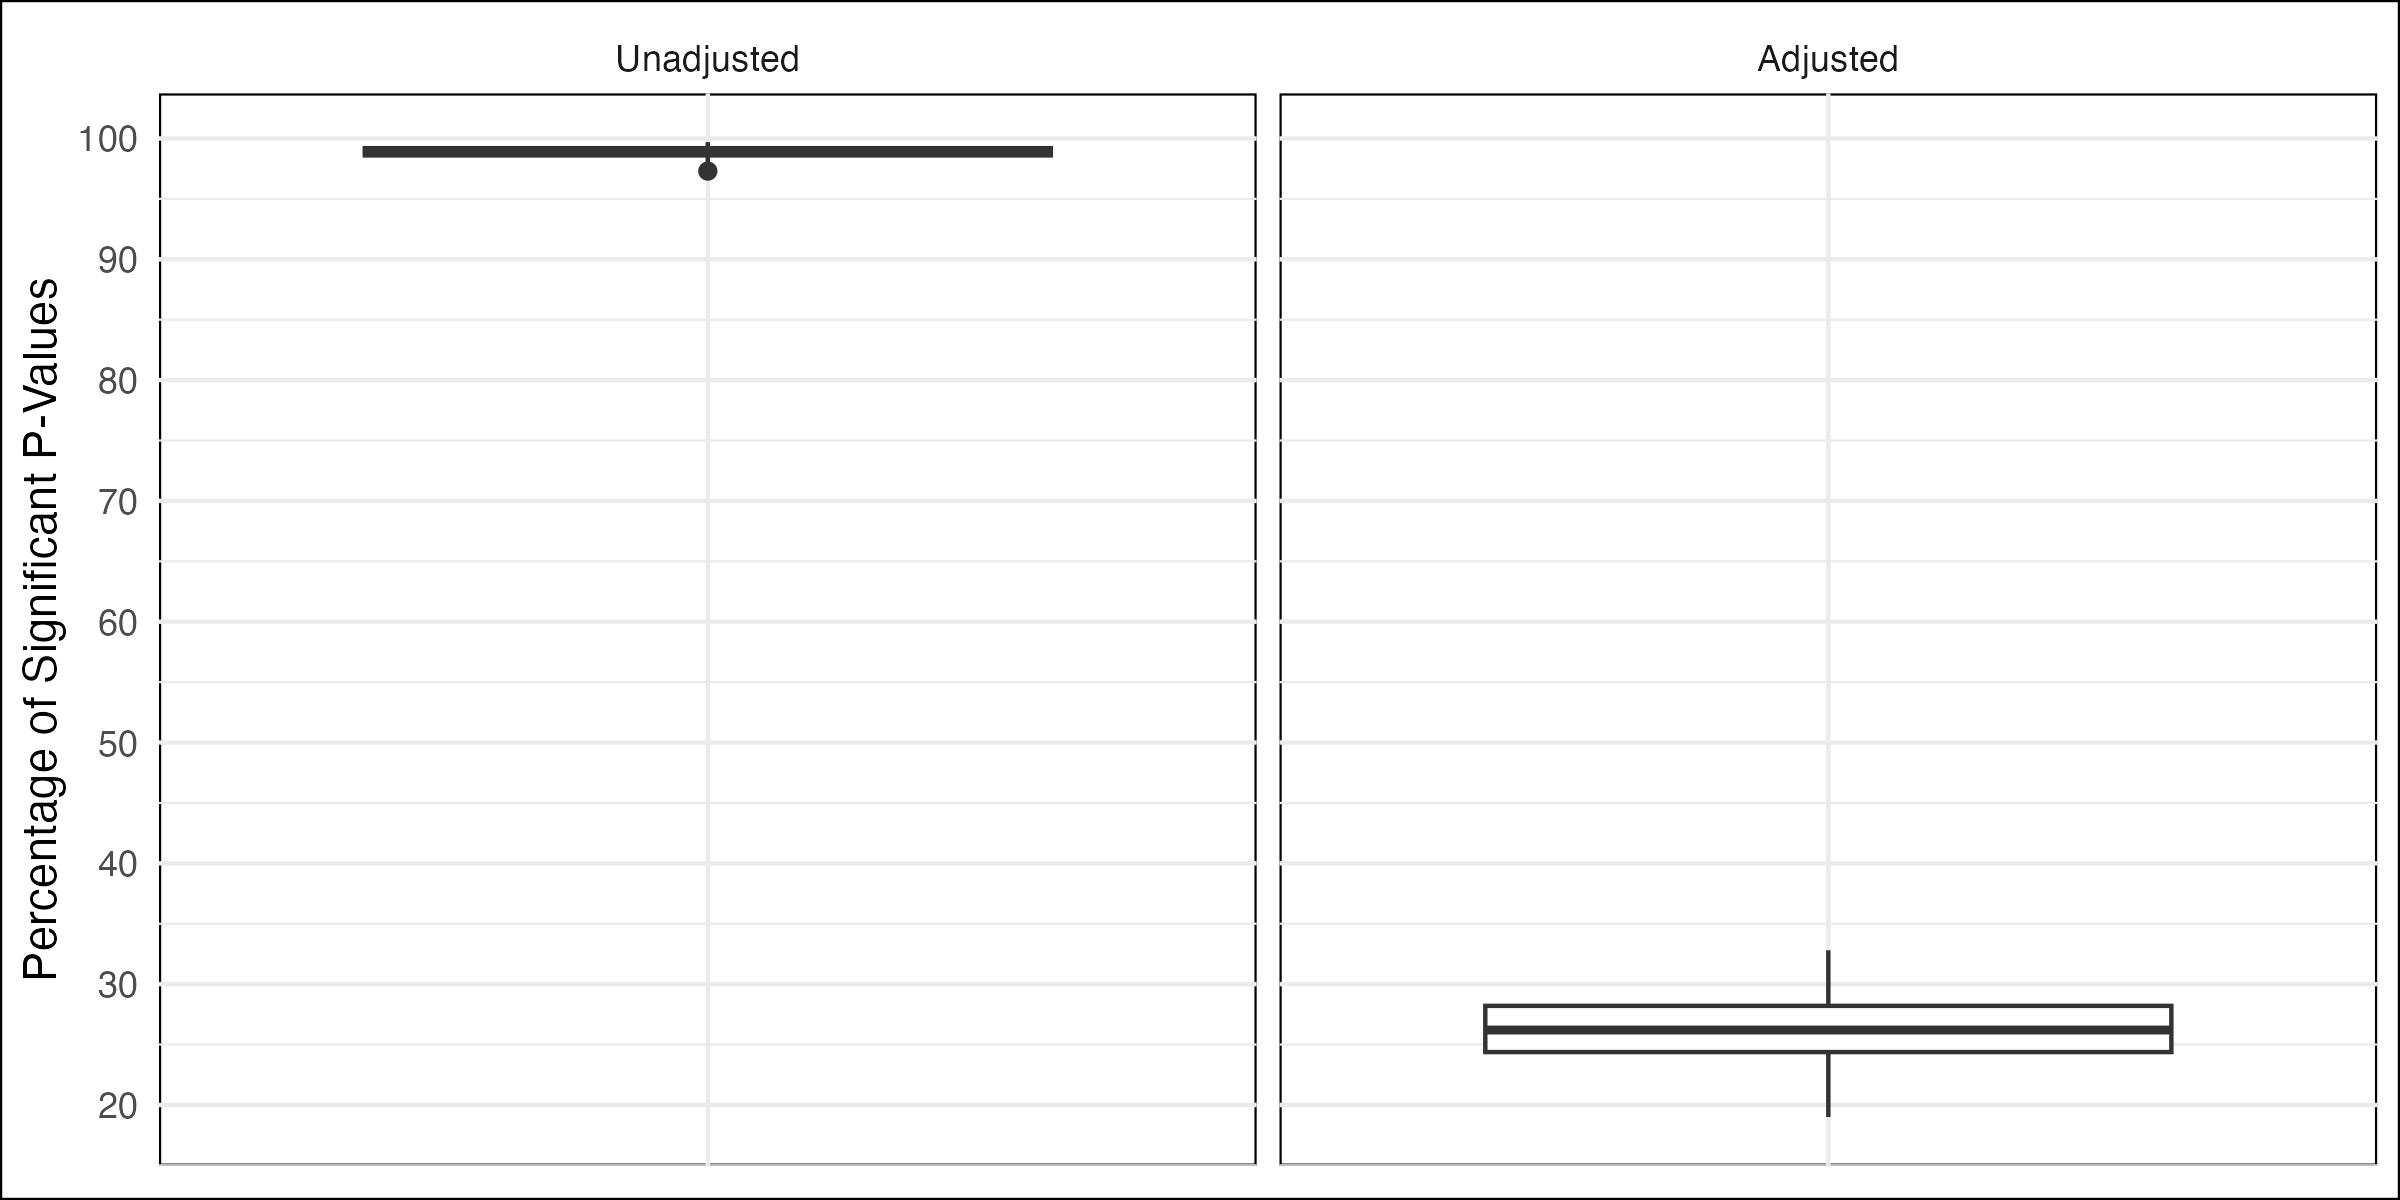
\includegraphics[width=\textwidth]{../Figures/lasso_boxplots.png}
  \caption{Percentage of significant p-values in outer area before (left) and after (right) adjustment from the LASSO models.}
  \label{fig:lasso_boxplot}
\end{figure}


\section*{Frequency}

The exponential correlation matrix with rate 1 was used to calculate the eigenvectors and eigenvalues. The matrix appeared to be positive-definite, so all eigenvalues were positive. These eigenvectors were then used to transform the pixel values. A Lasso regression model was fitted on the transformed data to predict \texttt{group\_ind}. To assess the significance of the model coefficients, 100 permutation tests were conducted within each iteration to obtain p-values. This process was replicated 100 times.

\clearpage

\section*{Simulation 1}

\begin{figure}[H]
  \centering
  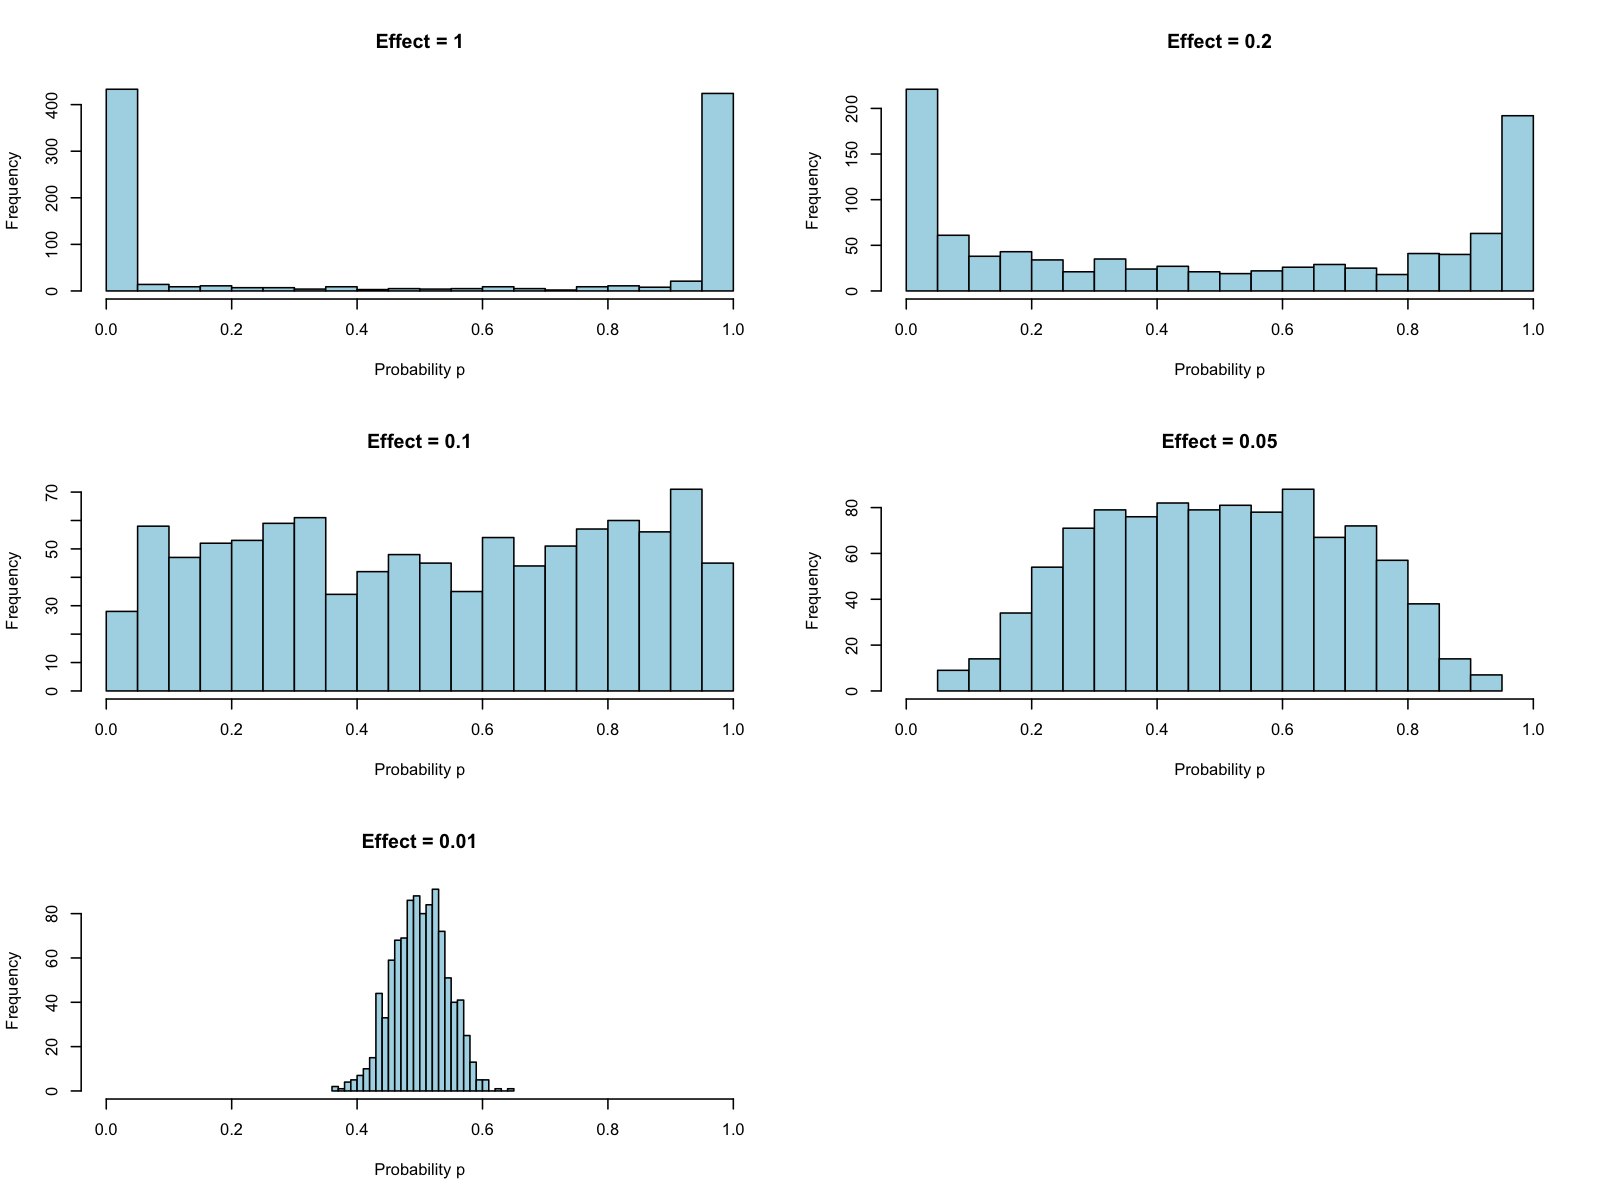
\includegraphics[width=\textwidth]{../Figures/sim1_p_dist.png}
  \caption{The distribution of \(p\) at different \(\beta\) values. \(\beta = 0.1\) was chosen for model fitting as it gives the most evenly distributed values.}
  \label{fig:sim1_p_dist}
\end{figure}

Figure~\ref{fig:sim1_p_dist} above shows the distribution of \(p\) for different values of \(\beta\). The choice of \(\beta = 0.1\) ensures an even spread of probabilities.

When using the \(\lambda\) given the lowest deviance and the lowest deviance plus 1 standard error, the average prediction accuracy on the test set is 72.5\% (min-max: 61.0\% - 82.0\%) and 72.2\% (59.0\% - 82.0\%). The corresponding AUC is 0.80 (SD=0.03) and 0.80 (SD=0.04). This indicates that the model is reasonably accurate and has a good discriminative ability.

\begin{figure}[H]
  \centering
  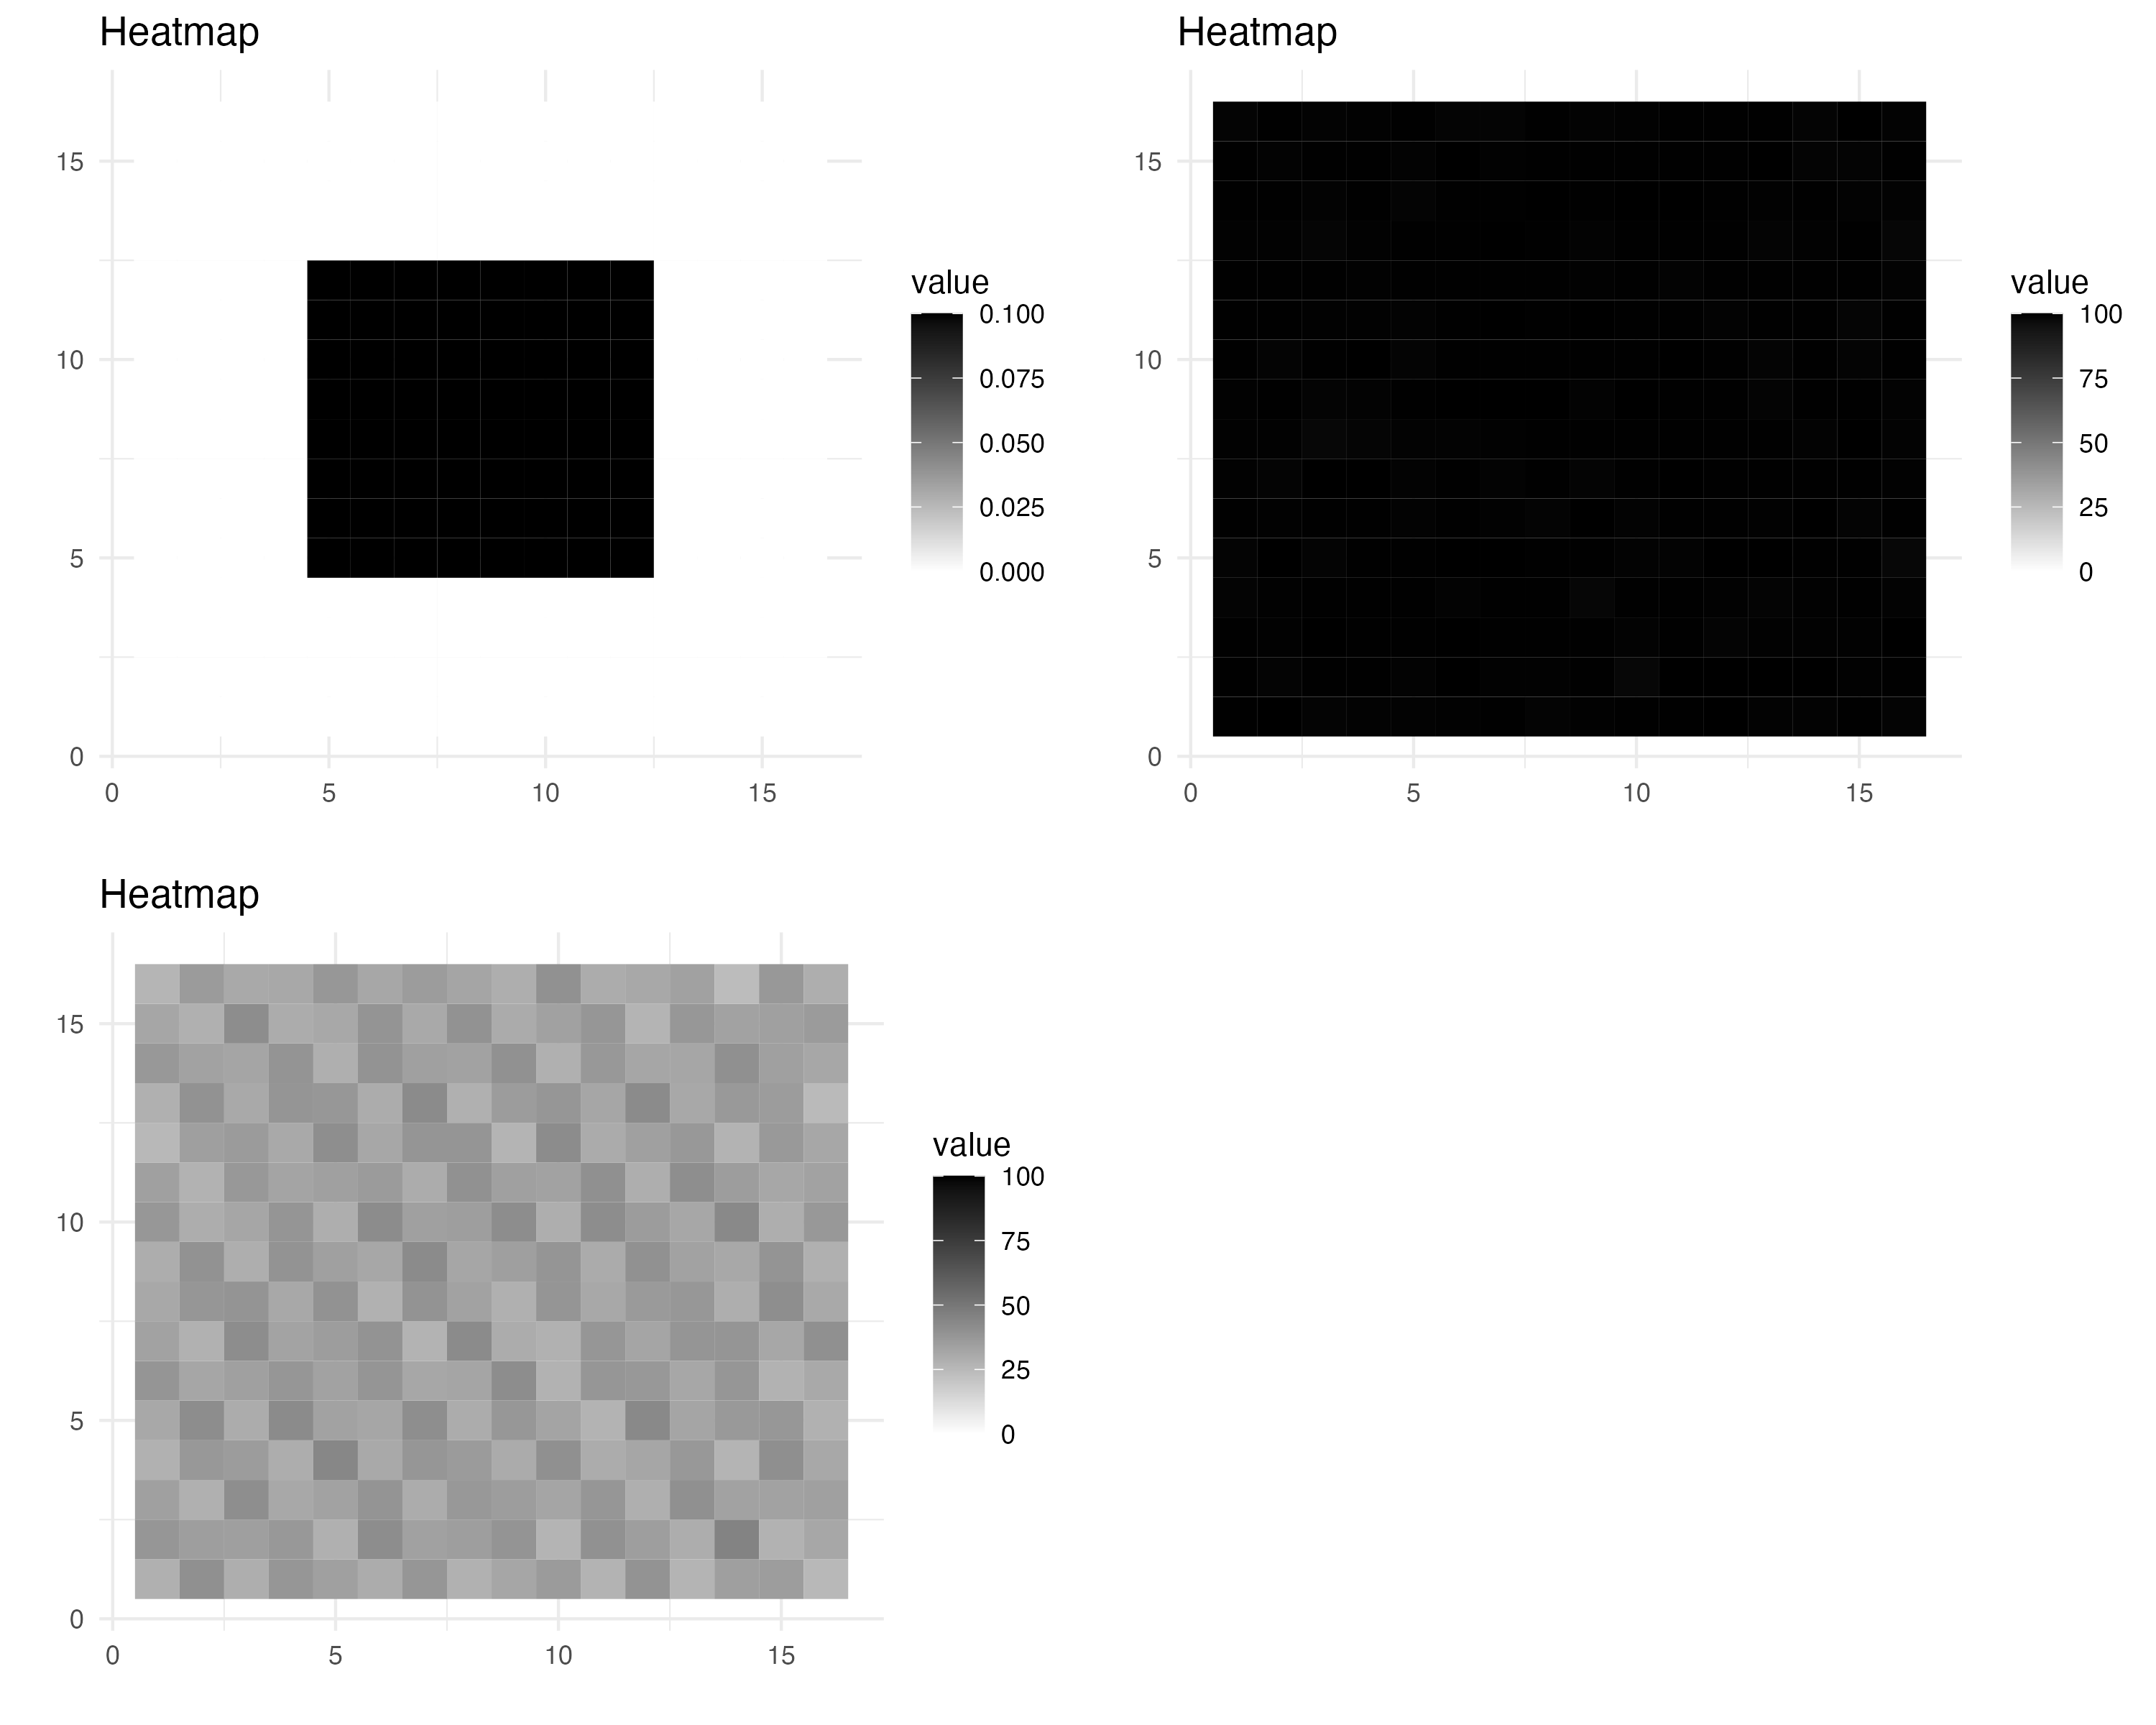
\includegraphics[width=\textwidth]{../Figures/sim1_heatmap.png}
  \caption{Heatmap of the actual \(\beta\) values, the percentage of getting a significant p-value for each pixel, and the percentage of getting a significant p-value after multiple comparisons adjustment.}
  \label{fig:sim1_heatmap}
\end{figure}

Figure~\ref{fig:sim1_heatmap} illustrates the true \(\beta\) values, the percentage of significant p-values, and the adjusted significance post-multiple comparisons. The results show that due to the correlation structure in \( X \), the LASSO model struggles to pinpoint the exact pixels with non-zero coefficients, resulting in diffuse significant p-values rather than precise identification.

\section*{Simulation 2}

Simulation 2 differs from Simulation 1 by transforming the covariate matrix into the frequency space using eigenvectors and assuming a sparse coefficient vector in this transformed space. The covariate matrix in the frequency space is generated with a multivariate normal distribution with diagonal values equal to 1 and all other values equal to 0. The coefficient vector index with non-zero values was randomly decided and 10\% elements are non-zero. The value of non-zero values was chosen similarly to Simulation 1.


\begin{figure}[H]
  \centering
  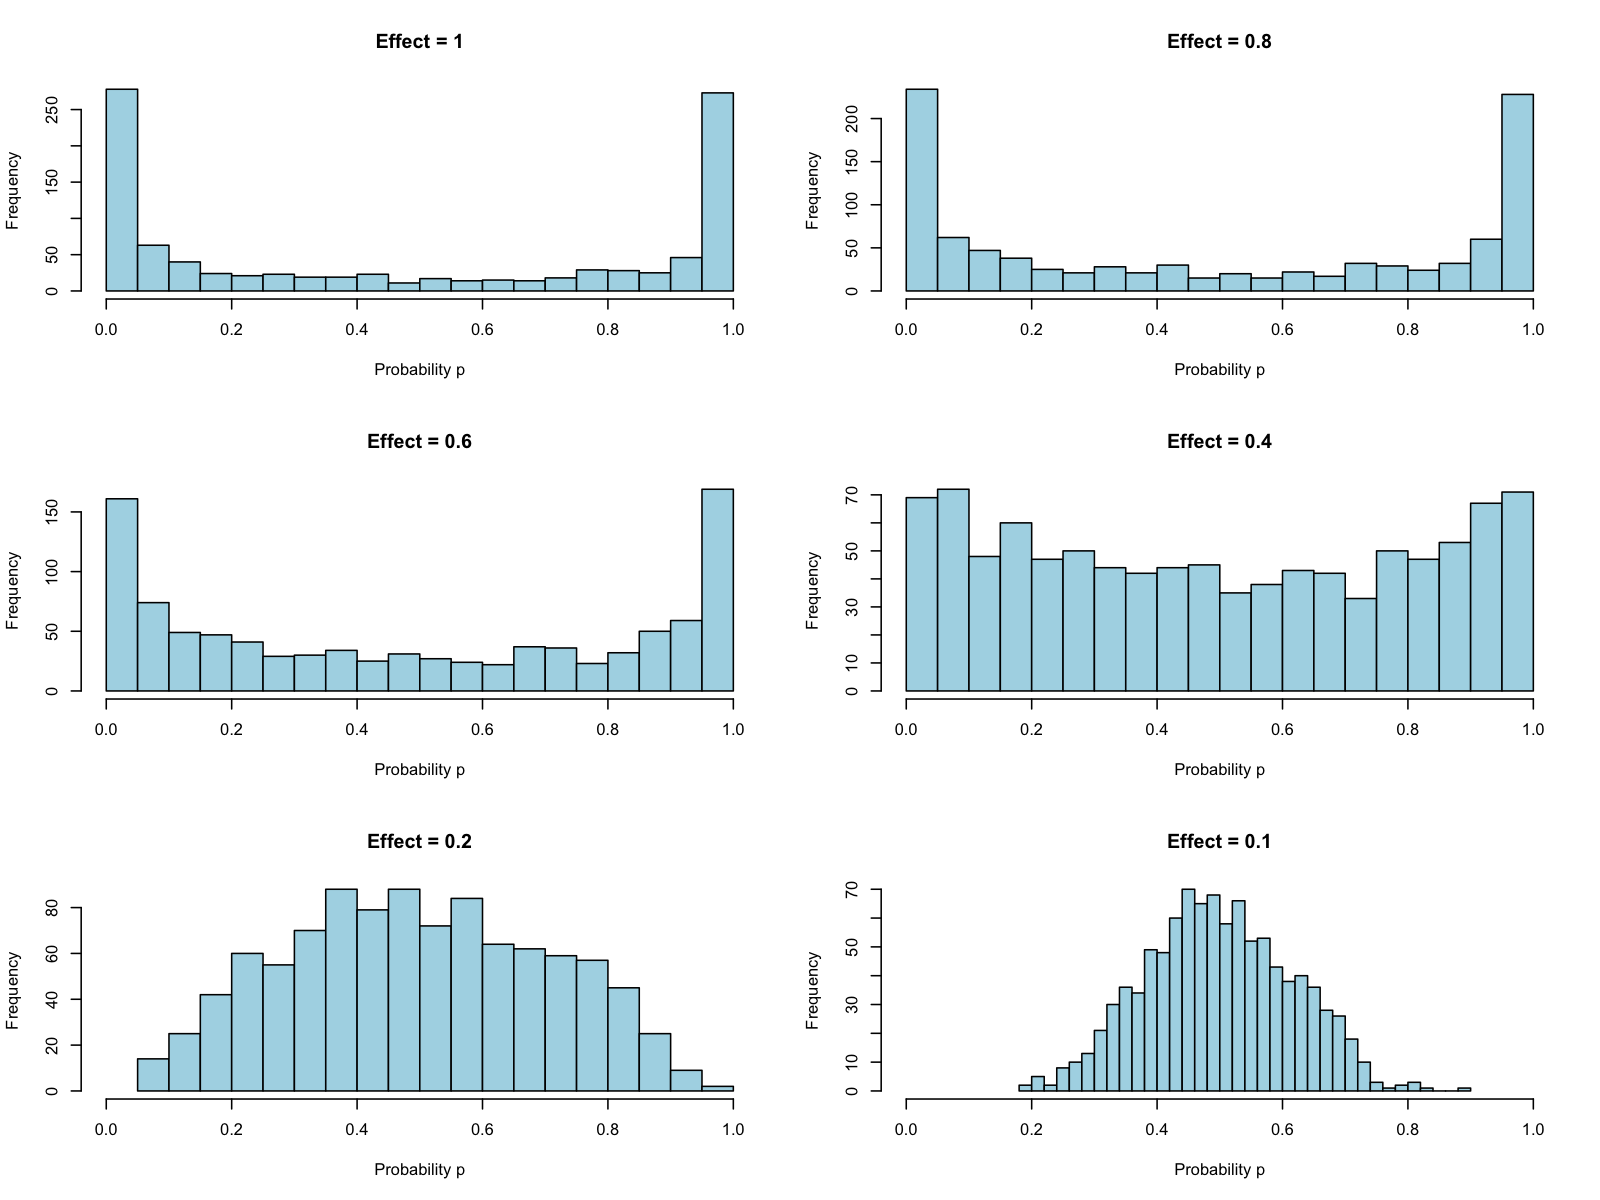
\includegraphics[width=\textwidth]{../Figures/sim2_p_dist.png}
  \caption{Distribution of \(p\) values in the frequency space when the non-zero value equals 0.4, showing a relatively balanced distribution.}
  \label{fig:sim2_p_dist}
\end{figure}

Figure~\ref{fig:sim2_p_dist} shows that when the non-zero value equals 0.4, the distribution of \(p\) values is relatively balanced, making it a suitable choice for the model.

Since the correlation between covariates was resolved by eigen-transpose, both accuracy and AUC are better than Simulation 1. The accuracy using the lowest deviance \(\lambda\) is 74.9\% (min-max, 66.0\% - 83.5\%), and 75.1\% (min-max, 65.5\% - 84.5\%) for \(\lambda\) for lowest deviance plus 1 standard error. The corresponding average AUC is 0.83 (SD 0.03) and 0.83 (SD 0.03). These results demonstrate that transforming the data into the frequency space can enhance model performance by reducing collinearity among covariates.

\begin{figure}[H]
  \centering
  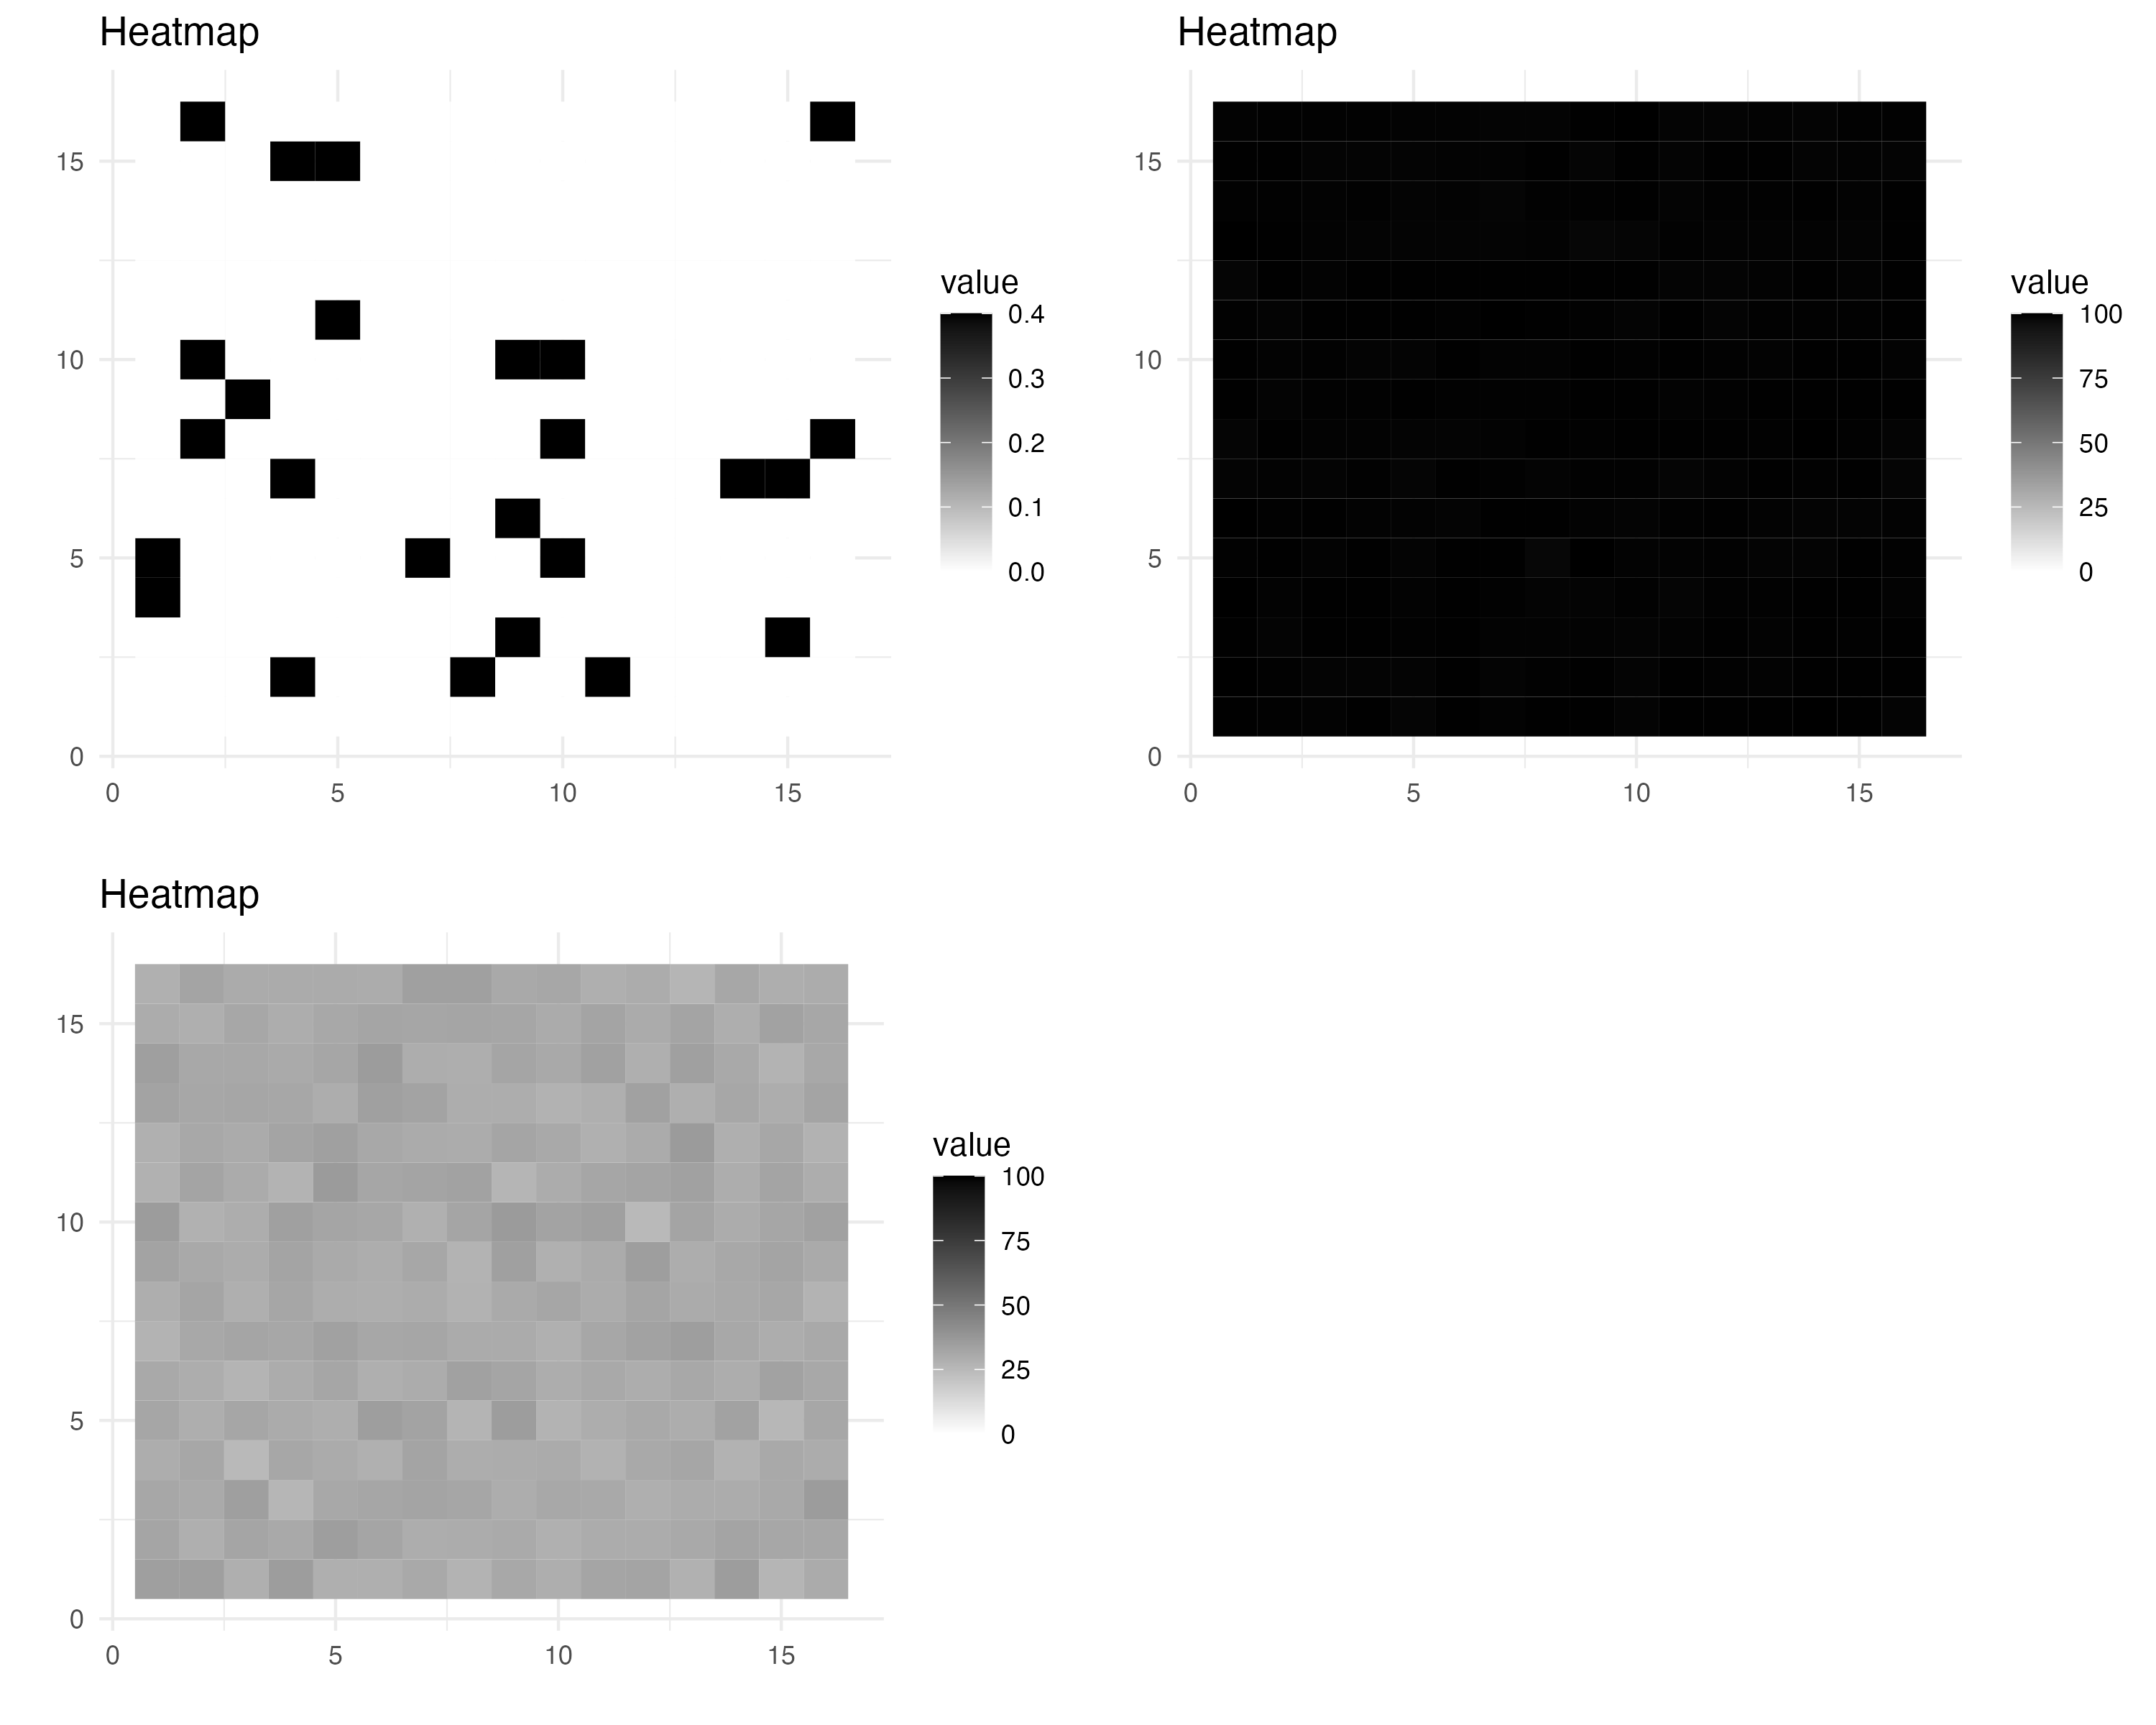
\includegraphics[width=\textwidth]{../Figures/sim2_heatmap.png}
  \caption{Heatmap of the coefficient vector in the frequency space, the percentage of getting a significant p-value for each pixel, and the percentage of getting a significant p-value after multiple comparisons adjustment.}
  \label{fig:sim2_heatmap}
\end{figure}

The heatmap for Simulation 2 (Figure~\ref{fig:sim2_heatmap}) shows the coefficient vector in the frequency space, significant p-values, and adjusted p-values. Despite the improvement in model performance, the heatmap reveals that the model still faces challenges in precisely identifying all non-zero coefficients.

\clearpage

\section*{Methods}

In this study, we conducted two simulations to evaluate the performace of LASSO models in identifying important features in high-dimensional data. The first simulation assumes sparsity of the features in the pixel space, while the second simulation assumes sparsity in the frequency space.

The pixel space refers to the original high-dimensional space where each dimension represents a pixel in an image. In this space, features are directly observed and may have inherent correlations. Conversely, the frequency space is a transformed version of the pixel space, obtained through techniques like eigen decomposition.

Suppose \( X \) is a column vector representing 256 pixels. Its covariance matrix, \( \Sigma \), is defined to have an exponential correlation structure, where \( \Sigma_{i j}=-\exp (\operatorname{dist}(i, j)) \). Here, \( \operatorname{dist}(i, j) \) is the distance between the pixels \( i \) and \( j \) in a \( 16 \times 16 \) matrix.

Let \( V \) be the matrix of eigenvectors of \( \Sigma \), with each column representing an eigenvector. We can transform the random vector \( X \) into the frequency space by \( X_{\text {freq }}=V^T X \). The covariance matrix of \( X_{\text {freq }} \) is given by \( \operatorname{cov}\left(X_{\mathrm{freq}}\right)=V^T \Sigma V \), which is a diagonal matrix.

For the simulations, in each iteration, we randomly generate \( X_{\text {freq }} \) from a multivariate normal distribution with the covariance matrix \(\ operatorname{cov}\left(X_{\text {freq }}\right) \). We repeat this process 1000 times. Then, we calculate \( X \) as \( X=V X_{\text {freq }} \).

In the first simulation, we assume sparsity in the coefficient vectors in the pixel space. The coefficient vector \( \beta \) was specified to have non-zero values exclusively within a central \( 8 \times 8 \) region. The response variable \( y \) was drawn from a binomial distribution with success probabilities determined by \( \eta = X \beta \). The non-zero coefficients in \( \beta \) were chosen such that the probability \( p = \frac{1}{1 + \exp(-\eta)} \) was uniformly distributed across interval \( [0, 1] \).

In the second simulation, we assume sparsity in the coefficient vectors in the frequency space. We defined a sparse coefficient vector \( b \) in the frequency space, where most of the 256 entries were zero and a randomly 10\% were non-zero. The response variable \( y \) was generated similarly to the first simulation, ensuring \( p = \frac{1}{1 + \exp(-\eta)} \) was evenly distributed.

For both simulations, we fit two models: one using the covariates in the pixel space and another using the covariates in the frequency space. Each dataset, generated in size \( 1000 \times 256 \) and representing images of \( 16 \times 16 \) pixels, was split into training (80\%) and test (20\%) sets. The regularization parameter \( \lambda \) was tuned using cross-validation with the default binomial deviance metric. The dataset was divided into 10 folds, with the model trained and validated iteratively across these folds, varying \( \lambda \). The optimal \( \lambda \) was chosen based on the lowest average binomial deviance.

After selecting the optimal \( \lambda \), model performance was evaluated using accuracy and AUC metrics. Additionally, a permutation test was conducted 100 times to calculate p-values for each covariate. Across all iterations, we calculated the mean and standard deviation of the metrics, as well as the percentage of significant p-values for each covariate.

\section*{Results}



\end{document}
